%%%%%%%%%%%%%%%%%%%%%%%%%%%%%%%%%%%%%%%%%%%%%%%%%%%%%%%%%%%%%%%
%% OXFORD THESIS TEMPLATE

% Use this template to produce a standard thesis that meets the Oxford University requirements for DPhil submission
%
% Originally by Keith A. Gillow (gillow@maths.ox.ac.uk), 1997
% Modified by Sam Evans (sam@samuelevansresearch.org), 2007
% Modified by John McManigle (john@oxfordechoes.com), 2015
% Modified by Ulrik Lyngs (ulrik.lyngs@cs.ox.ac.uk), 2018, for use with R Markdown
%
% Ulrik Lyngs, 25 Nov 2018: Following John McManigle, broad permissions are granted to use, modify, and distribute this software
% as specified in the MIT License included in this distribution's LICENSE file.
%
% John tried to comment this file extensively, so read through it to see how to use the various options.  Remember
% that in LaTeX, any line starting with a % is NOT executed.  Several places below, you have a choice of which line to use
% out of multiple options (eg draft vs final, for PDF vs for binding, etc.)  When you pick one, add a % to the beginning of
% the lines you don't want.


%%%%% CHOOSE PAGE LAYOUT
% The most common choices should be below.  You can also do other things, like replacing "a4paper" with "letterpaper", etc.

% This one will format for two-sided binding (ie left and right pages have mirror margins; blank pages inserted where needed):
%\documentclass[a4paper,twoside]{templates/ociamthesis}
% This one will format for one-sided binding (ie left margin > right margin; no extra blank pages):
%\documentclass[a4paper]{ociamthesis}
% This one will format for PDF output (ie equal margins, no extra blank pages):
%\documentclass[a4paper,nobind]{templates/ociamthesis}
%UL 2 Dec 2018: pass this in from YAML
\documentclass[a4paper, twoside]{templates/ociamthesis}


% UL 30 Nov 2018 pandoc puts lists in 'tightlist' command when no space between bullet points in Rmd file
\providecommand{\tightlist}{%
  \setlength{\itemsep}{0pt}\setlength{\parskip}{0pt}}
 
% UL 1 Dec 2018, fix to include code in shaded environments
\usepackage{color}
\usepackage{fancyvrb}
\newcommand{\VerbBar}{|}
\newcommand{\VERB}{\Verb[commandchars=\\\{\}]}
\DefineVerbatimEnvironment{Highlighting}{Verbatim}{commandchars=\\\{\}}
% Add ',fontsize=\small' for more characters per line
\usepackage{framed}
\definecolor{shadecolor}{RGB}{248,248,248}
\newenvironment{Shaded}{\begin{snugshade}}{\end{snugshade}}
\newcommand{\AlertTok}[1]{\textcolor[rgb]{0.94,0.16,0.16}{#1}}
\newcommand{\AnnotationTok}[1]{\textcolor[rgb]{0.56,0.35,0.01}{\textbf{\textit{#1}}}}
\newcommand{\AttributeTok}[1]{\textcolor[rgb]{0.77,0.63,0.00}{#1}}
\newcommand{\BaseNTok}[1]{\textcolor[rgb]{0.00,0.00,0.81}{#1}}
\newcommand{\BuiltInTok}[1]{#1}
\newcommand{\CharTok}[1]{\textcolor[rgb]{0.31,0.60,0.02}{#1}}
\newcommand{\CommentTok}[1]{\textcolor[rgb]{0.56,0.35,0.01}{\textit{#1}}}
\newcommand{\CommentVarTok}[1]{\textcolor[rgb]{0.56,0.35,0.01}{\textbf{\textit{#1}}}}
\newcommand{\ConstantTok}[1]{\textcolor[rgb]{0.00,0.00,0.00}{#1}}
\newcommand{\ControlFlowTok}[1]{\textcolor[rgb]{0.13,0.29,0.53}{\textbf{#1}}}
\newcommand{\DataTypeTok}[1]{\textcolor[rgb]{0.13,0.29,0.53}{#1}}
\newcommand{\DecValTok}[1]{\textcolor[rgb]{0.00,0.00,0.81}{#1}}
\newcommand{\DocumentationTok}[1]{\textcolor[rgb]{0.56,0.35,0.01}{\textbf{\textit{#1}}}}
\newcommand{\ErrorTok}[1]{\textcolor[rgb]{0.64,0.00,0.00}{\textbf{#1}}}
\newcommand{\ExtensionTok}[1]{#1}
\newcommand{\FloatTok}[1]{\textcolor[rgb]{0.00,0.00,0.81}{#1}}
\newcommand{\FunctionTok}[1]{\textcolor[rgb]{0.00,0.00,0.00}{#1}}
\newcommand{\ImportTok}[1]{#1}
\newcommand{\InformationTok}[1]{\textcolor[rgb]{0.56,0.35,0.01}{\textbf{\textit{#1}}}}
\newcommand{\KeywordTok}[1]{\textcolor[rgb]{0.13,0.29,0.53}{\textbf{#1}}}
\newcommand{\NormalTok}[1]{#1}
\newcommand{\OperatorTok}[1]{\textcolor[rgb]{0.81,0.36,0.00}{\textbf{#1}}}
\newcommand{\OtherTok}[1]{\textcolor[rgb]{0.56,0.35,0.01}{#1}}
\newcommand{\PreprocessorTok}[1]{\textcolor[rgb]{0.56,0.35,0.01}{\textit{#1}}}
\newcommand{\RegionMarkerTok}[1]{#1}
\newcommand{\SpecialCharTok}[1]{\textcolor[rgb]{0.00,0.00,0.00}{#1}}
\newcommand{\SpecialStringTok}[1]{\textcolor[rgb]{0.31,0.60,0.02}{#1}}
\newcommand{\StringTok}[1]{\textcolor[rgb]{0.31,0.60,0.02}{#1}}
\newcommand{\VariableTok}[1]{\textcolor[rgb]{0.00,0.00,0.00}{#1}}
\newcommand{\VerbatimStringTok}[1]{\textcolor[rgb]{0.31,0.60,0.02}{#1}}
\newcommand{\WarningTok}[1]{\textcolor[rgb]{0.56,0.35,0.01}{\textbf{\textit{#1}}}}
%UL 2 Dec 2018 add a bit of white space before and after code blocks
\renewenvironment{Shaded}
{
  \vspace{4pt}%
  \begin{snugshade}%
}{%
  \end{snugshade}%
  \vspace{4pt}%
}

%UL 2 Dec 2018 reduce whitespace around verbatim environments
\usepackage{etoolbox}
\makeatletter
\preto{\@verbatim}{\topsep=0pt \partopsep=0pt }
\makeatother

%UL 26 Mar 2019, enable strikethrough
\usepackage[normalem]{ulem}

%UL 15 Oct 2019, enable link highlighting to be turned off from YAML
\usepackage[colorlinks=false,pdfpagelabels,hidelinks=true]{hyperref}

%%%%% SELECT YOUR DRAFT OPTIONS
% Three options going on here; use in any combination.  But remember to turn the first two off before
% generating a PDF to send to the printer!

% This adds a "DRAFT" footer to every normal page.  (The first page of each chapter is not a "normal" page.)

% This highlights (in blue) corrections marked with (for words) \mccorrect{blah} or (for whole
% paragraphs) \begin{mccorrection} . . . \end{mccorrection}.  This can be useful for sending a PDF of
% your corrected thesis to your examiners for review.  Turn it off, and the blue disappears.
\correctionstrue

%%%%% BIBLIOGRAPHY SETUP
% Note that your bibliography will require some tweaking depending on your department, preferred format, etc.
% The options included below are just very basic "sciencey" and "humanitiesey" options to get started.
% If you've not used LaTeX before, I recommend reading a little about biblatex/biber and getting started with it.
% If you're already a LaTeX pro and are used to natbib or something, modify as necessary.
% Either way, you'll have to choose and configure an appropriate bibliography format...

% The science-type option: numerical in-text citation with references in order of appearance.
% \usepackage[style=numeric-comp, sorting=none, backend=biber, doi=false, isbn=false]{biblatex}
% \newcommand*{\bibtitle}{References}

% The humanities-type option: author-year in-text citation with an alphabetical works cited.
% \usepackage[style=authoryear, sorting=nyt, backend=biber, maxcitenames=2, useprefix, doi=false, isbn=false]{biblatex}
% \newcommand*{\bibtitle}{Works Cited}

%UL 3 Dec 2018: set this from YAML in index.Rmd
\usepackage[style=numeric-comp, sorting=none, backend=biber, doi=true, isbn=false]{biblatex}
\newcommand*{\bibtitle}{Bibliography}

% This makes the bibliography left-aligned (not 'justified') and slightly smaller font.
\renewcommand*{\bibfont}{\raggedright\small}

% Change this to the name of your .bib file (usually exported from a citation manager like Zotero or EndNote).
\addbibresource{bibliography/references.bib}


% Uncomment this if you want equation numbers per section (2.3.12), instead of per chapter (2.18):
%\numberwithin{equation}{subsection}


%%%%% THESIS / TITLE PAGE INFORMATION
% Everybody needs to complete the following:
\title{Lipids and dementia\\
An investigation of their relationship}
\author{Luke A McGuinness}
\college{}

% Master's candidates who require the alternate title page (with candidate number and word count)
% must also un-comment and complete the following three lines:
%\masterssubmissiontrue
%\candidateno{933516}
%\wordcount{28,815}

% Uncomment the following line if your degree also includes exams (eg most masters):
%\renewcommand{\submittedtext}{Submitted in partial completion of the}
% Your full degree name.  (But remember that DPhils aren't "in" anything.  They're just DPhils.)
\degree{Doctor of Philosophy in Population Health Sciences}
% Term and year of submission, or date if your board requires (eg most masters)
\degreedate{TBC}


%%%%% YOUR OWN PERSONAL MACROS
% This is a good place to dump your own LaTeX macros as they come up.

% To make text superscripts shortcuts
	\renewcommand{\th}{\textsuperscript{th}} % ex: I won 4\th place
	\newcommand{\nd}{\textsuperscript{nd}}
	\renewcommand{\st}{\textsuperscript{st}}
	\newcommand{\rd}{\textsuperscript{rd}}
	
	\definecolor{ashgray}{rgb}{0.7,0.75,0.71}

%%%%% THE ACTUAL DOCUMENT STARTS HERE
\begin{document}

%%%%% CHOOSE YOUR LINE SPACING HERE
% This is the official option.  Use it for your submission copy and library copy:
\setlength{\textbaselineskip}{22pt plus2pt}
% This is closer spacing (about 1.5-spaced) that you might prefer for your personal copies:
%\setlength{\textbaselineskip}{18pt plus2pt minus1pt}

% You can set the spacing here for the roman-numbered pages (acknowledgements, table of contents, etc.)
\setlength{\frontmatterbaselineskip}{17pt plus1pt minus1pt}

% UL: You can set the line and paragraph spacing here for the separate abstract page to be handed in to Examination schools
\setlength{\abstractseparatelineskip}{13pt plus1pt minus1pt}
\setlength{\abstractseparateparskip}{0pt plus 1pt}

% UL: You can set the general paragraph spacing here - I've set it to 2pt (was 0) so
% it's less claustrophobic
\setlength{\parskip}{2pt plus 1pt}


% Leave this line alone; it gets things started for the real document.
\setlength{\baselineskip}{\textbaselineskip}


%%%%% CHOOSE YOUR SECTION NUMBERING DEPTH HERE
% You have two choices.  First, how far down are sections numbered?  (Below that, they're named but
% don't get numbers.)  Second, what level of section appears in the table of contents?  These don't have
% to match: you can have numbered sections that don't show up in the ToC, or unnumbered sections that
% do.  Throughout, 0 = chapter; 1 = section; 2 = subsection; 3 = subsubsection, 4 = paragraph...

% The level that gets a number:
\setcounter{secnumdepth}{2}
% The level that shows up in the ToC:
\setcounter{tocdepth}{2}


%%%%% ABSTRACT SEPARATE
% This is used to create the separate, one-page abstract that you are required to hand into the Exam
% Schools.  You can comment it out to generate a PDF for printing or whatnot.
\begin{abstractseparate}
  \textbf{Background}\\
  In the UK, an estimated 800000 people are currently living with dementia and this number is expected to double
  by 2040. Despite the number of dementia cases and decades of research, there remains much unknown about
  the pathogenesis and progression of the disease, and, at present, no effective treatment exists to arrest or
  reverse the cognitive decline associated with the condition. In this context, identification of causal relationships
  between modifiable targets and dementia risk is central to the development of evidence-based prevention
  strategies and will be critically important in maintaining the long-term health of the ageing public. Blood lipid
  levels have been implicated in the aetiology of dementia by genetic linkage and functional cell biology studies,
  but current epidemiological evidence has yet to reach a consensus on their role in dementia risk.
\end{abstractseparate}

% JEM: Pages are roman numbered from here, though page numbers are invisible until ToC.  This is in
% keeping with most typesetting conventions.
\begin{romanpages}

% Title page is created here
\maketitle

%%%%% DEDICATION -- If you'd like one, un-comment the following.
\begin{dedication}
  For Brendan McHugh
\end{dedication}

%%%%% DECALRATION -- Nothing to do here except comment out if you don't want it.
\begin{declaration}
 	I declare that the work in this dissertation was carried out in accordance with the requirements of the University's Regulations and Code of Practice for Research Degree Programmes and that it has not been submitted for any other academic award. Except where indicated by specific reference in the text, the work is the candidate's own work. Work done in collaboration with, or with the assistance of, others, is indicated as such. Any views expressed in the dissertation are those of the author.

\begin{flushright}
SIGNED: ...................... \\
Luke McGuinness \\
Canynge Hall, Bristol \\
1 December 2021
\end{flushright}
\end{declaration}

%%%%% ACKNOWLEDGEMENTS -- Nothing to do here except comment out if you don't want it.
\begin{acknowledgements}
 	Additionally, I would like to thank Sharen O’Keefe.

Thanks to the creator of the oxfordown which was used

There are so many people without whom this would not have been possible:

{[}\textbf{Check all name spellings}{]}

Sharen O'Keffe
Neal Haddaway
Martin Westgate

robvis contributors

Statistical support:

All authors who volunteered time and effort

\begin{flushright}
Canynge Hall, Bristol \\
1 December 2021
\end{flushright}
\end{acknowledgements}

%%%%% ABSTRACT -- Nothing to do here except comment out if you don't want it.
\begin{abstract}
	\textbf{Background}\\
In the UK, an estimated 800000 people are currently living with dementia and this number is expected to double
by 2040. Despite the number of dementia cases and decades of research, there remains much unknown about
the pathogenesis and progression of the disease, and, at present, no effective treatment exists to arrest or
reverse the cognitive decline associated with the condition. In this context, identification of causal relationships
between modifiable targets and dementia risk is central to the development of evidence-based prevention
strategies and will be critically important in maintaining the long-term health of the ageing public. Blood lipid
levels have been implicated in the aetiology of dementia by genetic linkage and functional cell biology studies,
but current epidemiological evidence has yet to reach a consensus on their role in dementia risk.
\end{abstract}

%%%%% MINI TABLES
% This lays the groundwork for per-chapter, mini tables of contents.  Comment the following line
% (and remove \minitoc from the chapter files) if you don't want this.  Un-comment either of the
% next two lines if you want a per-chapter list of figures or tables.
  \dominitoc % include a mini table of contents

% This aligns the bottom of the text of each page.  It generally makes things look better.
\flushbottom

% This is where the whole-document ToC appears:
\tableofcontents

\listoffigures
	\mtcaddchapter
  	% \mtcaddchapter is needed when adding a non-chapter (but chapter-like) entity to avoid confusing minitoc

% Uncomment to generate a list of tables:
\listoftables
  \mtcaddchapter
%%%%% LIST OF ABBREVIATIONS
% This example includes a list of abbreviations.  Look at text/abbreviations.tex to see how that file is
% formatted.  The template can handle any kind of list though, so this might be a good place for a
% glossary, etc.
% First parameter can be changed eg to "Glossary" or something.
% Second parameter is the max length of bold terms.
\begin{mclistof}{List of Abbreviations}{3.2cm}

\item[1-D, 2-D] One- or two-dimensional, referring in this thesis to spatial dimensions in an image.

\item[Otter] One of the finest of water mammals.

\item[Hedgehog] Quite a nice prickly friend.

\end{mclistof} 


% The Roman pages, like the Roman Empire, must come to its inevitable close.
\end{romanpages}

%%%%% CHAPTERS
% Add or remove any chapters you'd like here, by file name (excluding '.tex'):
\flushbottom

% all your chapters and appendices will appear here
\hypertarget{covering-material}{%
\chapter*{Covering material}\label{covering-material}}
\addcontentsline{toc}{chapter}{Covering material}

\adjustmtc

Word count: 6969

Days: 15

Words behind: -1611

~

~

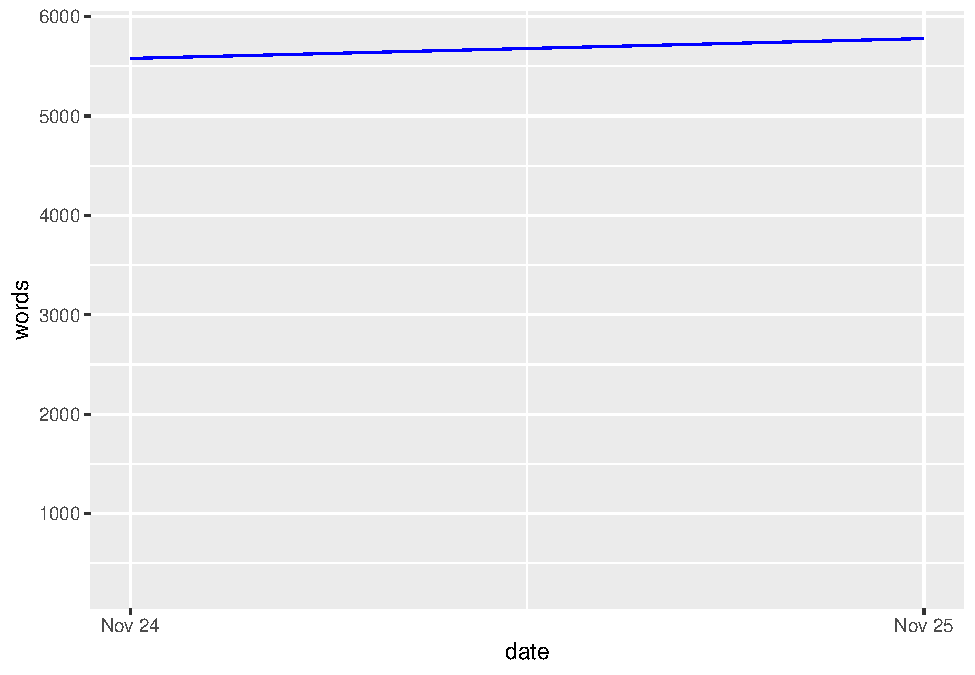
\includegraphics{_main_files/figure-latex/word-count-fig-1.pdf}

\hypertarget{intro-intro}{%
\chapter{Introduction}\label{intro-intro}}

\minitoc 

\hypertarget{additional-ideas}{%
\section{Additional ideas}\label{additional-ideas}}

\begin{itemize}
\tightlist
\item
  Explore difference/similarities between the published and unpublished literature, potentially formally, using funnel plots and also by following up preprints to see if they are eventually published. Limit to the date we ran the original search and see if any study included in the study had not been published by the time the review was finished.
\item
  Compare and contrast the codes used to find the AzD cases in the previous study and in this study, potentially with a view to contrasting misclassification between the two.
\end{itemize}

\hypertarget{aims-and-objectives-of-the-thesis}{%
\section{Aims and Objectives of the thesis}\label{aims-and-objectives-of-the-thesis}}

\hypertarget{aim}{%
\subsection{Aim}\label{aim}}

\hypertarget{objectives}{%
\subsection{Objectives}\label{objectives}}

\begin{itemize}
\tightlist
\item
  To review the published literature with respect to the effec tof lipids and lipid regulating agents\\
\item
  To examine whether there is evidence for an effect of lipid-regulating agents on dementia and related outcomes in a large scale population-based cohort, the Clinical Practice Research Datalink
\item
  To meta-analyze the
\end{itemize}

\hypertarget{chapter-overview}{%
\section{Chapter Overview}\label{chapter-overview}}

\begin{itemize}
\item
  \textbf{Chapter \ref{background-heading}:} Background information on dementia and blood lipid levels. This chapter provides an introduction to the topics covered in this thesis to non-subject area experts, and discusses the motivation for the remainder of the thesis.
\item
  \textbf{Chapter \ref{sys-rev-heading}} This Chapter describes a comprehensive systematic review and meta-analysis of all available evidence on the relationship between blood lipids and lipid
\item
  \textbf{Chapter \ref{cprd-analysis}:} This Chapter examines the relationship between lipid-regulating agent use and dementia outcomes in the Clinical Practice Research Datalink, a large primary care electronic health record database, based in England.
\item
  \textbf{Chapter @ref():} This Chapter seeks
\item
  \textbf{Appendix \ref{sys-rev-tools-heading}} This Chapter introduces new evidence synthesis two tools built in R: \texttt{robvis} and \texttt{medrixvr}. The motivation for, development and impact of, and future plans for these tools are outlined.
\end{itemize}

\hypertarget{thesis-output}{%
\section{Thesis Output}\label{thesis-output}}

The outputs of this thesis are detailed below, and include published peer review papers, presentations at conferences, open source evidence synthesis tools, and . . .

\hypertarget{peer-reviewed-papers}{%
\subsection{Peer reviewed papers}\label{peer-reviewed-papers}}

\textbf{Include other papers I have been involved in?}

\hypertarget{papers-under-review}{%
\subsection{Papers under review}\label{papers-under-review}}

\begin{itemize}
\tightlist
\item
  McGuinness et al.~
\end{itemize}

\hypertarget{software}{%
\subsection{Software}\label{software}}

A lot of packages were used in this project\textsuperscript{\protect\hyperlink{ref-base}{1}--\protect\hyperlink{ref-wordcountaddin}{14}}

\begin{itemize}
\item
  \texttt{robvis}: An R package and associated \texttt{shiny} web application that allows users to easily visualise the results of risk of bias graphs.
\item
  \texttt{medrxvir}: An R package and associated \texttt{shiny} web application that allows users to easily search and retrieve bibliographic data from the medRxiv\footnote{\url{https://www.medrxiv.org/}} preprint repository.
\end{itemize}

\hypertarget{talks}{%
\subsection{Talks}\label{talks}}

\begin{itemize}
\tightlist
\item
  Talk at Cochrane on medrxivr
\item
  Presentation to the
\item
  Webinar to Evidence Synthesis Ireland on Risk of Bias
\end{itemize}

\hypertarget{summary}{%
\section{Summary}\label{summary}}

\begin{itemize}
\item
\item
\item
\end{itemize}

\begin{savequote}
Science knows it doesn't know everything; otherwise, it'd stop
\qauthor{--- Dara O'Briain}\end{savequote}



\hypertarget{background-heading}{%
\chapter{Background}\label{background-heading}}

\minitoc 

\hypertarget{dementia}{%
\section{Dementia}\label{dementia}}

\hypertarget{definition-and-subtypes}{%
\subsection{Definition and Subtypes}\label{definition-and-subtypes}}

Dementia is major neurocognitive disorder, with symptoms including impairment of executive cognitive functions such as speech, judgement and memory. The most common causes of dementia are Alzheimer's disease and vascular dementia, accounting for \textasciitilde60-80\% and \textasciitilde10\% of cases respectively. The remaining 10-30\% of cases are caused other dementia subtypes (e.g.~Lewy Body dementia) or by progression of other neurological diseases (e.g.~Parkinson's disease).

\hypertarget{diagnosis}{%
\subsection{Diagnosis}\label{diagnosis}}

Dementia is difficult to diagnose, primarily due to the absence of a gold standard test for the condition. Information from multiple diagnostic tools are utilised, from medical history examination, through assessment of patients mental ability (e.g.~the Mini-Mental State Examination), to clinical tests (e.g.~Magnetic Resonance Imaging (MRI) scans).

\hypertarget{public-health-importance}{%
\subsection{Public Health Importance}\label{public-health-importance}}

Dementia is quickly becoming a critically important public health issue. Despite the age-specific incidence and prevalence of dementia remaining relatively constant over time,6 an ageing population looks set to create a dementia epidemic, particularly in Westernised countries. In the UK, there are estimated to be 800,000 people currently living with dementia, with this figure expected to double by 2040.7 Globally, the prevalence of dementia is expected to reach 75 million by 2030.8 Despite the number of dementia cases and decades of research, there remains much unknown about the pathogenesis and progression of the disease.

\hypertarget{challenges-in-the-study-of-dementia-using-traditional-study-designs}{%
\subsection{Challenges in the study of dementia using traditional study designs}\label{challenges-in-the-study-of-dementia-using-traditional-study-designs}}

Speak to the

Historically, studies on dementia have faced a range of challenges. As a range of determinants (genetic, environmental and lifestyle) are thought to jointly influence the risk, progression and outcomes of dementia, any individual association is likely to have only a small effect. Therefore, the statistical power need to detect these associations will often require sample sizes that are unfeasible using primary data collection.
This fact is further complicated by the long latency of dementia, which necessitates a costly long-term approach to patient follow-up. Furthermore, dementia studies often have limited generalisability to the target population, as certain subgroups (e.g.~the very old) are frequently under-represented in study cohorts due to difficulties associated with their recruitment.9 Finally, studies employing a case-control design are further limited by the high potential for differential recall bias between those who have and have not developed dementia.10

Fortunately, these limitations may potentially be addressed through the use of routinely collected health data, and the electronic health record databases in which they are stored.

Include CIND definition here

A further clinical subtype that is of particular import the

And MCI

And different scales

\hypertarget{history}{%
\subsection{History}\label{history}}

\begin{quote}
Two major clinical trials are often cited as providing evidence that statins do not have an effect on the incidence ofdementia: the Prospective Study ofPravastatin in the Elderly (PROSPER) and the Medical Research
Council/British Heart Foundation Heart Protection Study; however, because of methodologic limitations in relation to dementia outcomes in these two trials, the results of these trials are difficult to evaluate. Dementia incidence or cognitive outcomes were not preplanned endpoints in either of them, neither study included a clinical cognitive evaluation, and numbers of patients with follow-up information for cognitive evaluations were not reported in either study manuscript. In PROSPER a post hoc analysis compared changes in cognitive scores over a 3-year period between statintreated and placebo patients and found no significant differences. In the MRC/BHF HPS trial,27
similar percentages of participants (0.3\% in each---statin vs placebo---group) developed dementia during the 5-year follow-up period. The report did not state how the outcome of dementia was determined (e.g., reported as an adverse event or by follow-up phone interview).
\emph{Taken from Cramer 2008 - included in review}
\end{quote}

There exist only two large scale randomized controlled trials - in fact these studies are the only two trials included in a 2016 review of statins for the prevention of dementia produced by the Cochrane.\textsuperscript{\protect\hyperlink{ref-mcguinness2016b}{15}} Both showed no effect of

Queries around how the data were collected, along

\hypertarget{economic-impact}{%
\subsection{Economic impact}\label{economic-impact}}

\hypertarget{risk-factors}{%
\subsection{Risk factors}\label{risk-factors}}

\hypertarget{treatments}{%
\subsection{Treatments}\label{treatments}}

\hypertarget{preventative-measures}{%
\subsection{Preventative measures}\label{preventative-measures}}

\hypertarget{serum-lipids}{%
\section{Serum lipids}\label{serum-lipids}}

\hypertarget{range-of-lipids}{%
\subsection{Range of lipids}\label{range-of-lipids}}

\hypertarget{hdl-c}{%
\subsection{HDL-c}\label{hdl-c}}

\hypertarget{ldl-c}{%
\subsection{LDL-c}\label{ldl-c}}

\hypertarget{triglycerides}{%
\subsection{Triglycerides}\label{triglycerides}}

\hypertarget{total-cholesterol}{%
\subsection{Total cholesterol}\label{total-cholesterol}}

\hypertarget{serum-lipid-interventions}{%
\section{Serum lipid interventions}\label{serum-lipid-interventions}}

\hypertarget{statins}{%
\subsection{Statins}\label{statins}}

\hypertarget{lipophilic}{%
\subsubsection{Lipophilic}\label{lipophilic}}

\hypertarget{hydrophilic}{%
\subsubsection{Hydrophilic}\label{hydrophilic}}

\hypertarget{methods-used-in-the-thesis}{%
\section{Methods used in the thesis}\label{methods-used-in-the-thesis}}

\hypertarget{evidence-synthesis}{%
\section{Evidence synthesis}\label{evidence-synthesis}}

\hypertarget{triangulation}{%
\subsection{Triangulation}\label{triangulation}}

\hypertarget{individual-patient-data-meta-analyis}{%
\subsection{Individual patient data meta-analyis}\label{individual-patient-data-meta-analyis}}

\hypertarget{summary-1}{%
\section{Summary}\label{summary-1}}

\begin{savequote}
Why are open source statistical programming\\
languages the best?

Because they R.
\qauthor{--- Bealy, 2013\textsuperscript{\protect\hyperlink{ref-bealy2013}{16}}}\end{savequote}



\hypertarget{sys-rev-tools-heading}{%
\chapter{medrxivr: an R package for searching medRxiv and bioRxiv preprint data}\label{sys-rev-tools-heading}}

\minitoc 

\hypertarget{lay-summary}{%
\section{Lay summary}\label{lay-summary}}

Preprints are copies of academic manuscripts that are posted online in advance of being formally published by an academic journal.
They represent an important source of scientific literature.
A new software program called \texttt{medrxivr} was created as part of this thesis to allow researchers to find preprints related to their research in a transparent and reproducible way.
Development of this tool was required as part of this thesis, as preprints represent a key source of information needed for the research reported in future chapters.

\hypertarget{introduction}{%
\section{Introduction}\label{introduction}}

Preprints represent an increasingly important source of scientific information. Authors can use preprint servers for several purposes - to establish primacy when submitting to a journal where a the peer-review process may take several months; to post complete manuscripts that will never be formally published,{[}CITE{]} such as those reporting updated case reports during the COVID-19 pandemic;{[}CITE{]} and to make available publications that may not have been accepted elsewhere in an attempt to combat publication bias, or the ``file-drawer'' effect.

As a result, preprint repositories should be considered an distinct but complementary information source when reviewing the evidence base as part of a systematic review. The two key repositories in the health science are bioRxiv, established in 2013,\textsuperscript{\protect\hyperlink{ref-sever2019}{17}} and medRxiv, which evolved to replace the ``Epidemiology'' and ``Clinical Trial'' categories of bioRxiv, which launched in 2019.\textsuperscript{\protect\hyperlink{ref-rawlinson2019}{18}}

Preprints represent a particularly important to this thesis, ias one of the primary types of evidence that I planned to use in the triangulation exercise (Mendelian randomization (MR)) is still developing and many MR studies that look at the clinical question that this project aims to investigate are posted as preprints on the bioRxiv, and more recently medRxiv, preprint servers. Being able to systematically search these records for the purpose of the systematic review described in Chapter \ref{sys-rev-heading} was a necessity. In light of the above, the \texttt{medrxivr} R package was created in order to facilitate the searching of this data source.

In addition the

Developing new tools for facilitating evidence synthesis will benefit patients by speeding up the speed with which systematic reviews are produced. A recent study put the mean duration of a systematic review project, from date of registration to date of publication is 67.3 weeks.\textsuperscript{\protect\hyperlink{ref-borah2017}{19}} A large proportion of this time will be spent on manual tasks such as running searches and extracting records, title and abstract screening, and data extraction - therefore, efforts to increase the efficiency of the process should focus on process that can be automated.

In addition, we need to focus on developing tools that allow systematic, reproducible access to more informal sources of scientific material. One key emerging source

Searching pre-print repositories is becoming an increasingly important part of a systematic review. Preprints - unpublished versions of manuscripts, frequently uploaded to a repository at the same time they are submitted to a journal for peer review - represent an important source of grey literature. As the barriers and time to publication are both lower, they also represent an important source of information that may be either currently tied up in the peer-review process

At present, medRxiv allows only simple search queries, as opposed to the often complex Boolean logic that information specialists use to query other major databases. Additionally, record metadata (titles/abstracts/author lists) must be accessed individually, rather than in batches, meaning that downloading relevant records for title and abstract screening a time consuming task.

This chapter outlines the development and key functionality of \texttt{medrxivr\ (version\ 0.2)}. The motivating factors that necessitated the development of this tool as part of this thesis are discussed. The use of medrxivr in external projects and by other researchers is discussed. As the majority of work on this aspect of this thesis is represented by lines of code, this Chapter is a high-level summary. The GitHub repository for the \texttt{medrxivr} contains a complete record of the development of this tool, including discussion with other members of the systematic review community.

Current extraction mechanisms for extracting the results of searches from medRxiv are to go through each record, one-by-one, downloading individual citations. As the scale of the medRxiv database increases, particularly in light of the massive expansion as a result of COVID, this alreay time-consuming and error-prone method is not longer feasible.

\hypertarget{development}{%
\section{Development}\label{development}}

Work on this element began in Summer 2019, and initially existed as a collection of scripts built to allow for searching medRxiv and bioRxiv as part of the systematic search outline in Chapter \ref{sys-rev-heading}. Following interest from other researchers in using the ad-hoc web-scraping scripts, the initial version of the \texttt{medrxivr} package was released in February 2020. Additional development work took place, allowing for improved searching and exporting function

The updates to the systematic search to capture new literature published since the last search was performed with the fully developed package.

Early versions of the tool had a reliance on web-scraping data directly from the medRxiv website. Web-scraping is a fragile, or brittle, way to extract data, as it is entirely dependent on consistent website design and underlying code structure remaining unchanged.\textsuperscript{\protect\hyperlink{ref-shaw2002}{20},\protect\hyperlink{ref-laprie1992}{21}}.

However, an Application Programming Interface (API) for the medRxiv and bioRxiv repositories was released in early 2020, allowing for a newer version of the medrxivr package to engage in ``fault prevention'' and work towards a more robust interface with the available data.

Finally, while initial versions of the tool focused primarily on the medRxiv repository, discovery of some eligible required expansion to the bioRxiv repository, so that both can now be searched from a single tool. However, the introductory examples given below apply are taken from searches performed in the medRxiv repository.

Developed to meet three criteria:

\begin{enumerate}
\def\labelenumi{\arabic{enumi}.}
\tightlist
\item
  reproducible and transparent search functionality, with Boolean operator logic;\\
\item
  support for bulk export of references returned by the search;\\
\item
  automated access full-text records of relevant records.
\end{enumerate}

\hypertarget{installation}{%
\section{Installation}\label{installation}}

\texttt{medrxivr} has been released to the Comprehensive R Archive Network (CRAN), and can be installed with the following code

To install the stable \texttt{medrxivr} from CRAN:

~

\begin{Shaded}
\begin{Highlighting}[]
\KeywordTok{install.packages}\NormalTok{(}\StringTok{"medrxivr"}\NormalTok{)}
\end{Highlighting}
\end{Shaded}

~

Alternatively, the install the development version from GitHub:

\begin{Shaded}
\begin{Highlighting}[]
\CommentTok{# install.packages("devtools") }
\NormalTok{devtools}\OperatorTok{::}\KeywordTok{install_github}\NormalTok{(}\StringTok{"ropensci/medrxivr"}\NormalTok{)}
\end{Highlighting}
\end{Shaded}

The \texttt{medrxivr} R package is split into two component parts:

\begin{itemize}
\tightlist
\item
  An interface to the Cold Springs Harbor Laboratory API, which allows the wholesale import of the medRxiv and bioRxiv metadata
\item
  A collection of functions for working with the imported metadata, with an explicit focus on searching this data as part of a systematic review or evidence synthesis project.
\end{itemize}

The standard workflow is to download a copy of the preprint repository metadata, and then run your searchers locally. This is a workaround as the Cold Springs Harbor Labratory API does not provide any functionality to search the database.

\hypertarget{importing-preprint-meta-data}{%
\section{Importing preprint meta data}\label{importing-preprint-meta-data}}

\texttt{medrixvr} provides two ways to access medRxiv data.

\texttt{mx\_api\_content(server\ =\ "medrxiv")} creates a local copy of all data available from the medRxiv API at the time the function is run.

\begin{Shaded}
\begin{Highlighting}[]
\CommentTok{# Get a copy of the database from the live medRxiv API endpoint}
\NormalTok{preprint_data <-}\StringTok{ }\KeywordTok{mx_api_content}\NormalTok{()  }
\end{Highlighting}
\end{Shaded}

As an alternative to downloading a copy fo the database from the API in realtime, the \texttt{mx\_snapshot()} function provides access to a maintained static snapshot of the database. The snapshot is created each morning at 6am. This method, which doet not rely on the API, was created as during development e unavailable during peak usage times) and has the additional advantage of being faster, as it reads data from a comma-seperated file rather than having to re-extract it from the API.

The relationship between the two methods for accessing the data conatined in the medRxiv database is summarized in the figure below:

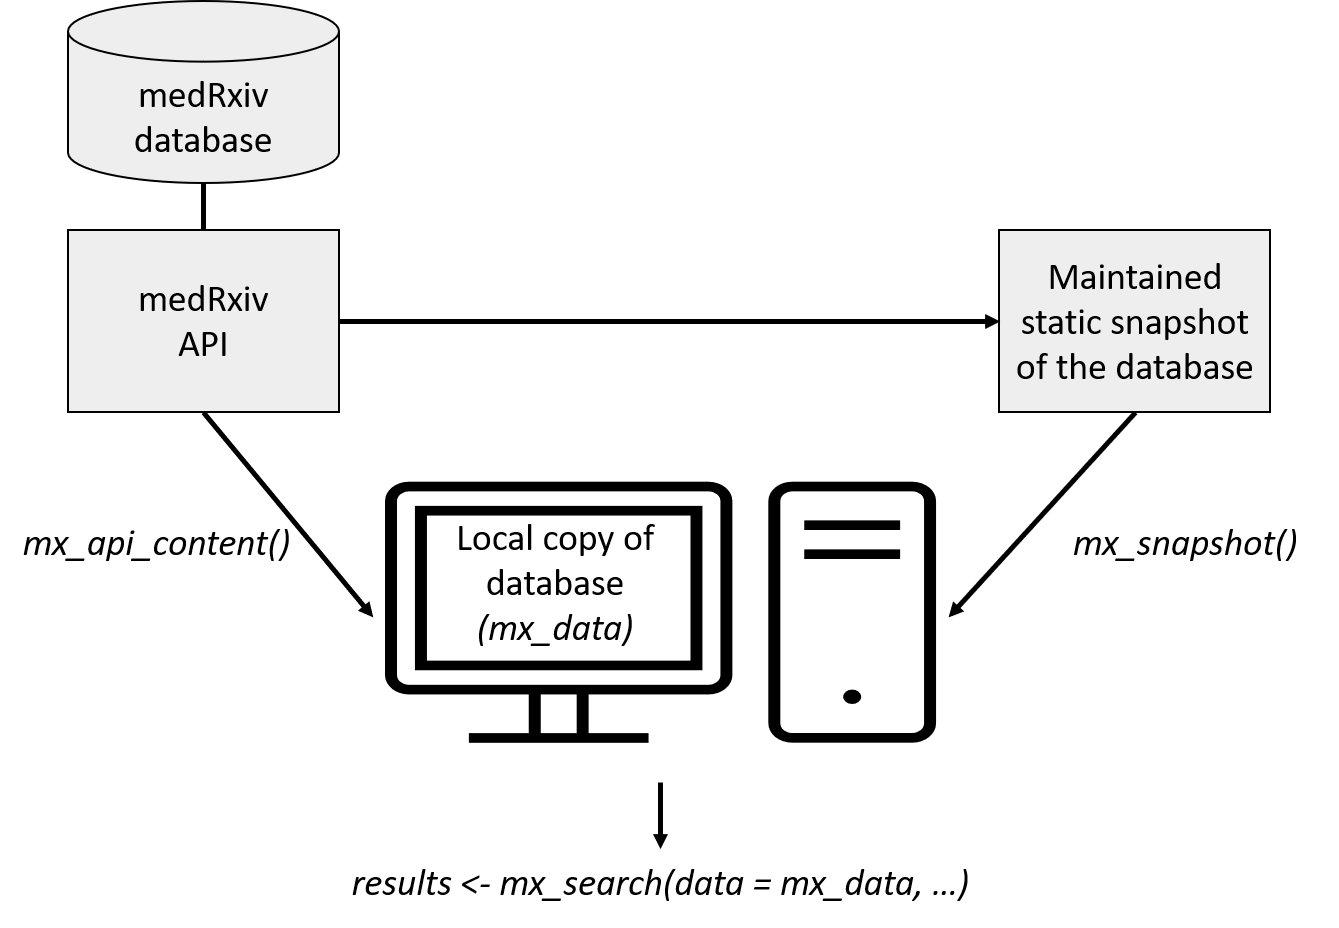
\includegraphics{figures/sys-rev-tools/data_sources.png}
\#\# Creating a search

Once a local copy of the database has been created, the functions in the \texttt{medrxivr} package then facilitate users in working with this dataset. There are two main functions and a helper function:

\begin{itemize}
\tightlist
\item
  \texttt{mx\_search()}: Enables users to search the preprint data, using regular expressions and Boolean logic.
\end{itemize}

~

\begin{Shaded}
\begin{Highlighting}[]
\NormalTok{topic1  <-}\StringTok{ }\KeywordTok{c}\NormalTok{(}\StringTok{"dementia"}\NormalTok{,}\StringTok{"alzheimer's"}\NormalTok{)  }\CommentTok{# Combined with OR}
\NormalTok{topic2  <-}\StringTok{ }\KeywordTok{c}\NormalTok{(}\StringTok{"lipids"}\NormalTok{,}\StringTok{"statins"}\NormalTok{)        }\CommentTok{# Combined with OR}

\NormalTok{myquery <-}\StringTok{ }\KeywordTok{list}\NormalTok{(topic1, topic2)         }\CommentTok{# Combined with AND}

\NormalTok{results <-}\StringTok{ }\KeywordTok{mx_search}\NormalTok{(myquery)}
\end{Highlighting}
\end{Shaded}

~

Additional functionality allowing common syntax used by systematic reviewers and health librarians, including the use of NEAR statements (which allows for ),

\hypertarget{further-functionality}{%
\section{Further functionality}\label{further-functionality}}

\hypertarget{exporting-to-bibliography}{%
\subsection{Exporting to bibliography}\label{exporting-to-bibliography}}

One of the key features of the \texttt{medrxivr} is the ability for users to export the results of their

For example, the results of our simple search above can be exported using the following code:

\begin{Shaded}
\begin{Highlighting}[]
\KeywordTok{mx_export}\NormalTok{(results, }
          \DataTypeTok{file =} \StringTok{"medrxiv_export.bib"}\NormalTok{)}
\end{Highlighting}
\end{Shaded}

\hypertarget{pdf-download}{%
\subsection{PDF download}\label{pdf-download}}

A second key use of the medrxivr package:

\begin{itemize}
\tightlist
\item
  \texttt{mx\_download()} Takes the output from \texttt{mx\_search()} and retrieves the full text PDF for each record, saving it to a folder specified by the user.
\end{itemize}

\begin{Shaded}
\begin{Highlighting}[]
\KeywordTok{mx_download}\NormalTok{(results,        }\CommentTok{# Object returned by mx_search()}
            \StringTok{"pdf/"}\NormalTok{)         }\CommentTok{# Directory to save PDFs to }
\end{Highlighting}
\end{Shaded}

\hypertarget{search-reporter}{%
\subsection{Search reporter}\label{search-reporter}}

One additional function creates a formatted output table with each search strategy presented on an individual line and the number of records associated with this strategy.

\begin{Shaded}
\begin{Highlighting}[]
\KeywordTok{mx_report}\NormalTok{(results)}
\end{Highlighting}
\end{Shaded}

This allows users to discover which aspects of their

\hypertarget{data-visualisation}{%
\subsection{Data visualisation}\label{data-visualisation}}

\hypertarget{shiny-app}{%
\subsection{Shiny app}\label{shiny-app}}

Part of the key theme of accessibility meant creating a web-application that allowed those without any knowledge of the R programming environment to benefit from it's functionality.
The app is readily available and has

\hypertarget{reception-and-future-plans}{%
\section{Reception and future plans}\label{reception-and-future-plans}}

The tool has be well received by the community (as of December 2020, \texttt{medrxivr} has been downloaded more than 1000 times, and the medRxivr app has been visited more than ????), and several use cases have been reported. It has been used to visualize the growing number of preprints related to the 2019 coronavirus outbreak,\footnote{\url{https://twitter.com/L_Brierley/status/1233109086444695553}} perform systematic searches in a number of other systematic reviews,\textsuperscript{\protect\hyperlink{ref-noone2020}{22}} in addition to forming a platform for an analysis of researcher's differing data-sharing tendencies under two different journal models (preprint server vs formal publication).{[}CITE{]}

Following rigorous peer-review, it has been onboarded into the rOpenSci suite of packages, a collection of ``carefully vetted, staff- and community-contributed R software tools that lower barriers to working with scientific data sources on the web'', and an associated article published in the Journal of Open Source Software.\textsuperscript{\protect\hyperlink{ref-mcguinness2020a}{23}} The entire review discussion is publicly available and can be viewed online.\footnote{\url{https://github.com/ropensci/software-review/issues/380}}

Lobbying of the cold springs harbour labratory has been ongoing. This would negate the current need to download a full copy of the relevant preprint database before searching it locally, which is currently the rate limiting step for.

\hypertarget{comparison-with-other-search-options}{%
\section{Comparison with other search options}\label{comparison-with-other-search-options}}

During development of the package, there were several alternative considered as part of a audit of existing tools. However, development of a new custom tool was preferred as none met the three criteria required: 1) reproducible and transparent search functionality, with Boolean operator logic; 2) support for bulk export of references returned by the search; 3) automated access full-text records of relevant records.

Some previous tools exist while allowed for robust searching of preprint repositories, such as \texttt{search.bioPreprint}\textsuperscript{\protect\hyperlink{ref-iwema2016}{24}}- however, these tools were aimed more at those looking to keep up to date with recent developments rather than systematically assess the entirety . As such, they did not support needed functionality such as bulk export of records matching a search term, unlimited return of records (c.f. \texttt{search.bioPreprint} which is limited to the most recent 1000 records matching a user search).

\hypertarget{package-infrastructure}{%
\section{Package infrastructure}\label{package-infrastructure}}

The \texttt{medrxvir} package was written in R using RStudio, and followed development best practices, including complete and information documentation, a robust unit testing framework (99\% of all code lines within the package are formally tested under this framework) across multiple platforms including Windows, MacOS, and Linux, and in-depth code review by two experienced reviewers.

The medRxiv snapshot is still taken every morning using GitHub Actions, an automated system for repetitive tasks.

An automatically generated documentation website is also generated on each update to the code-base\footnote{\url{https://docs.ropensci.org/medrxivr/}}

\hypertarget{discussion}{%
\section{Discussion}\label{discussion}}

Packaging and sharing R scripts should be a fundamental part of evidence synthesis process. {[}{]}

While searching of the medRxiv database was crucical for the systematic review element of this thesis presented in Chapter \ref{sys-rev-heading}

\textbf{Need to also touch on the biases involved in search preprint literature, in that the authors of those in the }

it is too early to see if preprint reps

There is the potential that the cross-section of literature posted on medrxiv would be substantially different from the true grey literature - simply lowering the barriers to publication may encourage authors to published ``null'' results,{[}CITE{]} but due to the effort involved in writing up a distributable manuscript, it is unlikely to completely address the ``file drawer'' effect.{[}CITE{]}

As

By implementing the tool described above as both as an R package and a \texttt{Shiny} web app, the functionality is available to evidence synthesists with varying levels of ability in R. These tools serve as an example of the advantages of ``packaging'' the R scripts that evidence synthesists often create for personal use.\textsuperscript{\protect\hyperlink{ref-wickham2015r}{25}} In the case of \texttt{medrxivr}, it is likely that several other evidence synthesists had written scripts that have a similar functionality - in fact, in the course of its development, one other researcher that has done so was identified. This duplication of time and effort is inefficient, and creating and sharing well-documented R packages represents one way to reduce this inefficiency. Taking this approach one step further, \texttt{Shiny} apps represent a straightforward way to provide a user-friendly GUI for a newly created R package within a very short time-frame, expanding the potential pool of users of the package to anyone with an internet connection.

Creating a package using R has a number of advantages unique to the R programming environment. R provides access to a range of powerful tools including the \texttt{ggplot} infrastructure for creating publication-quality plots, and RMarkdown, which enables creation of documents that can be rendered in a range of formats such as PDF, HTML, or Word.\textsuperscript{\protect\hyperlink{ref-xie2018r}{26}} Furthermore, and focusing specifically on evidence synthesis, building new tools as packages in R allows for easy integration with the range of existing evidence synthesis packages. Recently, the \texttt{metaverse} project,\textsuperscript{\protect\hyperlink{ref-variousauthors2020}{27}} of \texttt{medrivr} is a part, has begun to curate a collection of R packages that cover different aspects of the systematic review and meta-analysis process which, when taken together, form a coherent end-to-end open-source alternative to commercial offerings such as Covidence or Review Manager. Key offerings in this suite of packages include \texttt{litsearcher}, which facilitates systematic search strategy development, \texttt{revtools}, a package for managing the review process and performing title and abstract screening, \texttt{metaDigitise}, a package for automatic extraction of data from figures in research papers, and \texttt{metafor}, a package for conducting meta-analyses in R.\textsuperscript{\protect\hyperlink{ref-grames2019automated}{28}--\protect\hyperlink{ref-westgate2019revtools}{31}}

\hypertarget{summary-2}{%
\section{Summary}\label{summary-2}}

\begin{itemize}
\item
  In this Chapter, I have introduced a new tool, \texttt{medrxivr}, for performing complex searches in the medRxiv and bioRxiv preprint repositories.
\item
  I have outlined the motivation for developing this tool in relation to this thesis - more specifically, that it was used to perform systematic and reproducible searches of a key literature source used in the comprehensive systematic review described in Chapter \ref{sys-rev-heading}.
\item
  The impact of this tool to date, its place in the broader evidence synthesis in R ecosystem, and a roadmap for its future development has been discussed.
\end{itemize}

\begin{savequote}
Science knows it doesn't know everything; otherwise, it'd stop
\qauthor{--- Dara O'Briain}\end{savequote}

--- Dara O'Briain --- Dara O'Briain

\hypertarget{sys-rev-heading}{%
\chapter{Systematic Review}\label{sys-rev-heading}}

\minitoc 

\hypertarget{lay-summary-1}{%
\section{Lay summary}\label{lay-summary-1}}

\hypertarget{additional-ideas-1}{%
\section{Additional ideas}\label{additional-ideas-1}}

\begin{itemize}
\tightlist
\item
  Evidence map - show the distribution of the different studies population across the world.
\item
  Living systematic review approach - update weekly based on medRxiv
\end{itemize}

\hypertarget{aims}{%
\section{Aims}\label{aims}}

The aim of this chapter is to systematically review all available literature on the association between blood levels of total cholesterol and it's constituent parts (HDL-c,LDL-c and triglycerides) on the subsequent risk of dementia.

Based on the review of prev, no previous

Literature con

\hypertarget{methods}{%
\section{Methods}\label{methods}}

\hypertarget{search-strategy}{%
\subsection{Search strategy}\label{search-strategy}}

We will systematically search electronic bibliographic databases to identify potentially relevant records. The search strategy used in each database will be developed in an iterative manner using a combination of free text and controlled vocabulary (MeSH/EMTREE) terms to identify studies which have examined the relationship between blood lipids levels and dementia, incorporating input from an information specialist. The strategy will include terms related to lipids, lipid modifying treatments, and dementia and its sub-types, and will be designed for MEDLINE before being adapted for use in the other bibliography databases listed. An outline of the general strategy is presented in the Table 3.2 below and the full draft search strategies for each database are attached to this protocol. To ensure that the study design filters are not excluding potentially relevant records, a random sample of 500 records identified by the main search but excluded by the filters (defined as Line 7 NOT Line 13 in Table 3.2) will be screened. If any potentially relevant studies are identified, their titles and abstracts will be searched for key terms that can be incorporated into the filters to improve search sensitivity.

The following databases will be searched from inception onwards: Medline, EMBASE, Psychinfo, Cochrane Central Register of Controlled Trials (CENTRAL), and Web of Science Core Collection. We will also search clinical trial registries, for example ClinicalTrials.gov, to identify relevant randomized controlled trials.

The abstracts list of relevant conferences (e.g.~the proceedings of the Alzheimer's Association International Conference, published in the journal Alzheimer's \& Dementia) will be searched. Grey literature will also be searched via ProQuest, OpenGrey and Web of Science Conference Proceedings Citation Index, while theses will be accessed using the Open Access Theses and Dissertations portal. We will also search bioRxiv and medRxiv, preprint repositories using a tool built as part of this thesis, to identify potentially relevant studies. Finally, the reference lists of included studies will be searched by hand while studies citing included studies will be examined using Google Scholar (forward and reverse citation searching).

\hypertarget{study-selection}{%
\subsection{Study selection}\label{study-selection}}

Records will be imported into Endnote and deduplicated using the method outlined in Bramer et al.~(2016).\textsuperscript{\protect\hyperlink{ref-bramer2016}{32}} Screening (both title/abstract and full-text) will be performed using a combination of Endnote and Rayyan, a web based screening application.\textsuperscript{\protect\hyperlink{ref-ouzzani2016}{33}}
Title and abstract screening to remove obviously irrelevant records will be performed by the primary author, with a random selection of excluded records being screened in duplicate to ensure consistency with the inclusion criteria. If this demonstrates a significant level of erroneous exclusion by the primary author a larger proportion will be dual-screened.
Full-text screening will also be completed in full by the primary author. A second reviewer will screen a random sample of included and excluded records, in addition to any records identified by the first reviewer as being difficult to assess against the inclusion criteria. Reasons for exclusion at this stage will be recorded. Disagreements occurring during either stage of the screening process will be resolved through discussion with a senior colleague. A PRIMSA flow diagram will be produced to document how records moved through the review.\textsuperscript{\protect\hyperlink{ref-zotero-766}{34}}

\hypertarget{inclusion}{%
\subsubsection{Inclusion}\label{inclusion}}

We will seek studies that examine the relationship between blood lipid levels (or any specific lipid fraction, including total cholesterol, HDL, LDL, and triglycerides) and risk of incident dementia/MCI. Eligible study designs include randomized controlled trials and non-randomized observational studies of lipid modifying treatments, longitudinal studies examining the effect of increased/decreased blood lipid levels, and genetic instrumental variable (Mendelian randomization) studies examining the effect of genetically increased/decreased blood lipid levels.

Participants will be free (or assumed to be free) of dementia/MCI at baseline. Studies of any duration will be included to allow for exploration of the effect of length of follow-up on the effect estimate using meta-regression. No limits will be placed on the sample size of included studies.

Eligible studies will define dementia according to recognised criteria, for example the National Institute of Neurological Disorders and Stroke Association-Internationale pour la Recherche en l'Enseignement en Neurosciences (NINDS-AIREN), International Classification of Diseases (ICD), or Diagnostic and Statistical Manual of Mental Disorders (DSM) criteria. For MCI, eligible studies are those that attempted state a definition for diagnoses of MCI (e.g.~an adapted version of the Petersen criteria\textsuperscript{\protect\hyperlink{ref-petersen1999}{35}}) and create ordinal groups of patients (e.g.~no dementia or dementia/MCI/dementia) based on this definition.

No limitations will be imposed on publication status, publication date, venue or language, although we will require sufficiently detailed reports of the studies to be able to examine their methods. Preprints and unpublished reports will be eligible for inclusion if relevant. Multiple publications resulting from the analysis of the same data will be included and grouped.

\hypertarget{exclusion}{%
\subsubsection{Exclusion}\label{exclusion}}

Case-control studies, cross-sectional studies, qualitative studies, case reports/series and narrative reviews will be excluded. Studies which present no evidence of attempting to exclude prevalent cases from their analyses will also be excluded. Studies that measure change in continuous cognitive measures (e.g.~MoCA score) without attempt to map these scores to ordinal groups (e.g.~no dementia/MCI/dementia) will be excluded. Conference abstracts with no corresponding full-text publication will be examined, and we will contact authors to obtain information on the study's status. Studies that are reported in insufficient detail (e.g.~only in conference abstracts, new, letters, editorials and opinion) will be excluded. Previous systematic reviews will not be eligible, but their reference lists will be screened to identify any potentially relevant articles. Studies with outcomes not directly related to the clinical syndrome of dementia (e.g., neuroimaging), studies implementing a ``multi-domain intervention'' where the lipid-regulating agent is included in each arms (e.g.~for example, a study examining exercise + statins vs statins alone, but a study examining exercise + statins vs exercise alone would be included), and studies where there was no screening for dementia at baseline except if the sample was initially assessed in mid-life (i.e.~below the age of 50) will be excluded.

Excluded studies performing autopsy unless it was done under accepted criteria
Exclude studies using a dietary intervention, for example omega-3 fatty acid enriched diet, as it hard to disentangle the effect of other elements contained within te diet, vs simple tablet based supplements of

\hypertarget{data-extraction}{%
\subsection{Data extraction}\label{data-extraction}}

Harmonization of cholesterol measures across studies was performed, as different studies used different methods to quantify exposure, including comparing differing risks in the highest vs lowest quartiles of a lipid, using a binary classification of patients into a hypercholesterolaemia or not, categorising lipid levels into high, middle, and low groups according to study-defined criteria, and simply treating the exposure as a continuous variable.

\hypertarget{risk-of-bias-assessment}{%
\subsection{Risk of bias assessment}\label{risk-of-bias-assessment}}

Risk of bias assessment was performed using the domain-based risk-of-bias assessment tool appropriate to the study design. Randomised controlled trials were assessed using the RoB2 tool,\textsuperscript{\protect\hyperlink{ref-sterne2019}{36}}, non-randomised studies of interventions were assessed using the ROBINS-I tool,\textsuperscript{\protect\hyperlink{ref-sterne2016}{37}} and non-randomised studies of exposures were assessed using the ROBINS-E tool.{[}TBC{]}

At present, no risk of bias assessment tool for Mendelian randomisation studies is available. Bias in thesee studies was assessed with the help of an expert panel {[}TBC{]}

Data will be visualized using a paired forest and risk of bias plot

\hypertarget{patient-and-public-involvement}{%
\subsection{Patient and public involvement}\label{patient-and-public-involvement}}

\hypertarget{results}{%
\section{Results}\label{results}}

\hypertarget{screening-results}{%
\subsection{Screening results}\label{screening-results}}

Following screening, XXX studies were included.

The distribution of included studies over time demonstrates that despite the conduct of several previous reviews of different types of literature surrounding this question, primary studies continue to the published as these reviews have yet to provide a definite answer.

Table \ref{tab:incl-studies-character} shows the characteristics {[}\textbf{Include column here that says whether it was included in a systematic review - see below}{]}

\emph{As part of our our forward snowballing exercise (where articles citing an included study are cited), we recorded whether a study included in our review had been included in any previous evidence synthesis attempt in an attempt to qualify the added value of this analysis. Additionally, if an included article was subsequently cited by a review, all studies in that review were screened for inclusion for the sake of completeness. This analysis was performed by extracting the citing articles from Google Scholar on XXXX and screening them manually. The DOI of articles extracted from this analysis are included in the appendix, as the Google Scholar search functionality is not readily reproducible.}

As a summary of the duplication of work in this area, we looked at how many reviews a single included study had previously been included in.

\hypertarget{inter-rater-reliability}{%
\subsubsection{Inter-rater reliability}\label{inter-rater-reliability}}

Inter- and intra-rater reliability was asssessed for a 10\% subsample of records at the title and abstract screening stage. Intra-rater reliability involved a sinlge reviewer applying the inclusion criteria to the same set of records while blinded to their previous decisions, while inter-rater reliability involved two reviewers independently screening the same set of records.

Rater reliability was assessed using Gwet's agreement coefficient (AC1).\textsuperscript{\protect\hyperlink{ref-gwet2008}{38}} This measure of inter-rater reliabilty was chosen over other methods of assessing inter-rater reliability such as percent agreeement (number of agreements divided by total number of assessments) as i account for chance agreement between reviewers but does not suffer from severely imbalanced marginal totals in the same way that Cohen's kappa value does. {[}\protect\hyperlink{ref-cohen1960}{39}:\textsuperscript{\protect\hyperlink{ref-gwet2008}{38},\protect\hyperlink{ref-wongpakaran2013}{40}}

How to interpret agreement co-efficients is widely debated. Here we use guidelines based on a stricter interpreation of the Cohen's Kappa coefficient,\textsuperscript{\protect\hyperlink{ref-mchugh2012}{41}} presented in Table \ref{tab:gwettable}.

In a two by two table with cells A, B, C and D, Gwet's AC1 is calculated using the following:

\[AC1 = \frac{p-e(\gamma)}{1-e(\gamma)}\]
Here, \(p = \frac{A+D}{N}\) and \(e(\gamma)\) is the chance agreement between raters, given as \(2q(1-q)\), where \(q = \frac{(A+C)+(A+B)}{2N}\)

-\textgreater{} Insert formula here. Need to be sure of how to calculate.\textsuperscript{\protect\hyperlink{ref-gwet2008}{38},\protect\hyperlink{ref-sim2005}{42}}

\begin{table}

\caption{\label{tab:agreementtableinter}Inter-rater reliability}
\centering
\begin{tabular}[t]{>{}l>{}lr>{}r|r}
\toprule
\multicolumn{2}{c}{ } & \multicolumn{3}{c}{Initial screening descision} \\
\cmidrule(l{3pt}r{3pt}){3-5}
 &  & Exclude & Include & Total\\
\midrule
 & \textbf{Exclude} & 1244 & 9 & 1253\\
\cmidrule{2-5}
 & \textbf{Include} & 26 & 22 & 48\\
\cmidrule{2-5}
\multirow{-3}{*}{\raggedright\arraybackslash \textbf{Second reviewer decision}} & \textbf{Total} & 1270 & 31 & 1301\\
\bottomrule
\end{tabular}
\end{table}

\begin{table}

\caption{\label{tab:agreementtableintra}Intra-rater reliability}
\centering
\begin{tabular}[t]{>{}l>{}l|r>{}r|r}
\toprule
\multicolumn{2}{c}{ } & \multicolumn{3}{c}{Initial screening decision} \\
\cmidrule(l{3pt}r{3pt}){3-5}
 &  & Exclude & Include & Total\\
\midrule
 & \textbf{Exclude} & 1266 & 14 & 1280\\
\cmidrule{2-5}
 & \textbf{Include} & 4 & 17 & 21\\
\cmidrule{2-5}
\multirow{-3}{*}{\raggedright\arraybackslash \textbf{Same reviewer decision}} & \textbf{Total} & 1270 & 31 & 1301\\
\bottomrule
\end{tabular}
\end{table}

For the inter-rater reliability, percentage agreement was 97.3\% (AC1 = XXXX, Table \ref{tab:agreement-table-intra}), while for the intra-rater reliability, agreement was 98.6\% (AC1 = XXXX, Table \ref{tab:agreement-table-intra}).

The discrepancy between the percent agreement and the associated value of AC is expected, due to the heavy imbalance in this sample towards exclusion.\textsuperscript{\protect\hyperlink{ref-feinstein1990}{43}}

Those records which were excluded in the initial screening, but were included either by the same reviewer on their second viewing (n=4), or by the second reviewer (n=29), were investigated. This discrepancy between the two reviewers was explained in all cases by differing interpretations of the inclusion criteria, specifically around the definition of cognitive decline vs mild cognitive impairment and the definition of eligible lipids.

\hypertarget{prisma-flowchart}{%
\subsubsection{PRISMA flowchart}\label{prisma-flowchart}}

Following de-duplication, the titles and abstracts of 16109 records were assessed for eligibility. 387 were deemed potentially eligible and the full text records for these were requested and screened. {[}\textbf{CROSS-REF to PRISMA flow here}{]}

A breakdown of records by

\hypertarget{included-studies}{%
\section{Included studies}\label{included-studies}}

XXXX studies met the criteria for inclusion in the review.

Include here:

\begin{itemize}
\item
  PRISMA Flowchart (use PRISMA2020 from GitHub - depending on level of involvement, could refer to the Appendix here too.)
\item
  Summary of types of study
\item
  Summary of locations
\item
  Summary of diagnostic criteria used
\item
  Summary of risk of bias
\item
  Long table, horizontally. Newer version of flextable (GH) allows for PDF output
\end{itemize}

\hypertarget{publication-bias}{%
\section{Publication bias}\label{publication-bias}}

\begin{itemize}
\tightlist
\item
  Check if there are protocols available for any of the published reports, and whether there were
\item
  Vascular dementia has substantially less published reports. Many (reference Smeeth et al 2010 here) simply group into AD and non-AD making comparison between published st
\end{itemize}

\hypertarget{triangualtion-across-evidence-sources}{%
\subsection{Triangualtion across evidence sources}\label{triangualtion-across-evidence-sources}}

One key question for which multiple distinct sources of evidence were available were those looking at Laz

A key limitiation for other types of dementia, in particularly vascular, is that there has yet to be a GWAS identifying relevant SNPS that could then be used in a MR study with SNPS for lipids to estimates the causal effect of lipids on vascular dementia {[}\textbf{Is this true?}{]} This rules out the use

\hypertarget{discussion-1}{%
\section{Discussion}\label{discussion-1}}

Of note, as part of the review, we identified serveral previous systematic reviews of this topic. However, this review is the firest to

\hypertarget{conclusion}{%
\section{Conclusion}\label{conclusion}}

\begin{savequote}
``When dealing with human beings controlled experiments frequently prove
to be impracticable, so for a scientific basis for our assumptions we
turn to past history to reconstruct the suspected causal chain of events
- and then our statistical troubles may begin''
\qauthor{--- Harold F. Dorn, 1953\textsuperscript{\protect\hyperlink{ref-dorn1953}{44}}}\end{savequote}



\hypertarget{cprd-analysis}{%
\chapter{Primary analysis of lipid regulating agents and dementia}\label{cprd-analysis}}

\minitoc 

\hypertarget{additional-ideas-2}{%
\section{Additional ideas}\label{additional-ideas-2}}

One of the problems I'll point out with the trials in the systematic review chapter (Chapter \ref{sys-rev-heading}) is that they only included people with a high cardiovascular risk - we are kind of doing the same by using elevated test cholesterol results as the index event.

Might be able to get around this by pointing out

\hypertarget{things-we-tried}{%
\section{Things we tried}\label{things-we-tried}}

\begin{itemize}
\tightlist
\item
  Conditioning entry to the cohort on QRISK score (as defined by codes) rather than. Need to be able to demonstrate here that not many meeting our original entry criteria actually go on to have a statin quickly. Need total number of those starting and average time to start.
\item
  Positive controls. Need to be able to explain why these controls have such wildly increased results.
\item
  Competing risk analysis, with death as a competing risk. Need numbers of deaths in each group, and preliminary results
\item
  Allowing for time-varying confounders for binary covariates.
\item
  Replicating a matched analysis a la Smeeth et al 2010 - though questions were raised as to how they had actually done the analysis (they did not match on propensity score, they simply adjusted for it - find paper that explores 4 ways of accounting for PS and shows this is the worst), they adjusted for things likely to be on the causal pathway, and they saw a huge change in direction for MI pre- vs post- adjustment.
\end{itemize}

\hypertarget{things-we-could-try}{%
\section{Things we could try}\label{things-we-could-try}}

\begin{itemize}
\tightlist
\item
  Work through data using positive control to see if the way it is being added is what is causing the issues.
\item
  Examine Cramer et al.~thesis and see what they did
\item
  Marginal structural models approach (a la J. Sterne)
\end{itemize}

\hypertarget{aims-1}{%
\section{Aims}\label{aims-1}}

In this

\hypertarget{methods-1}{%
\section{Methods}\label{methods-1}}

\hypertarget{estimation-methods}{%
\subsection{Estimation methods}\label{estimation-methods}}

Potential biases included time varying confounding, selection bias due to censoring on death and
We performed a Cox test this si to addd some words.

\hypertarget{estimating-the-value-of-the-time-varying-confounders}{%
\subsection{Estimating the value of the time-varying confounders}\label{estimating-the-value-of-the-time-varying-confounders}}

Mean time from index event to first prescription of statins was 2.4 years. This negates the promised benefit of ruling out confounding by indication (where the test result leads to the prescription of the treatment and also increases the risk of the outcome, distorting the relationship between the two), as there is no relationship between index TC/LDL-c and eventual LRA prescription.

Additionally, the time between index event and prescription does lead to a problem in terms of time varying confounding, as an average time of 2.4 years between current measurement of the covariates and treatment switching means there is plenty of time for the value of the covariate to change. This is problematic when the descision to change treatments (in this case to move from no LRA use to LRA use) is influenced by a set of prognostic factors that in turn may have been influenced by the inital treatment decision, as is likely to be the case for a range of covariates included in the model. For example:

\begin{verbatim}
_No CVD (t=0) -> No LRA (t=0) -> CVD (t=1) -> LRA (t=1) -> Dementia (t=2)_
\end{verbatim}

In this case, the decision to move to LRA use is influenced by CVD status at \emph{Time 1}, which will not be captured by adjusting only for CVD status at \emph{Time 0}.

In practice, this means that the value of the prognostic factor should be regularly captured

However, in electronic health records, a change in the value of the prongostic factors is only important if it is recorded in a patients record, as for it to have an impact on treatment decisions, it must be recorded.

This means we can find the most recent value of the covariate before the switch and apply a marginal structural model approach, filling all values for that variable before the most recent measure with the baseline measurement, and all after the most recent meausure with the value of the most recent measure (on the basis that you won't go from having CVD back to not having CVD).

i.e.\\
Timepoint 12345678\\
CVD 00001111\\
Treatment 00000111

Split into 3 month blocks since index event and use the same approach as above to work out the values of each covariate at each time point.

Note: this will be harder for things that are not dichotomous and can go up as well as down. Examples include total cholesterol and BMI, which can go up as well as down.

\hypertarget{the-effect-of-total-cholesterol-or-ldl-cholesterol-on-lra-prescription}{%
\subsection{The effect of total cholesterol or LDL-cholesterol on LRA prescription}\label{the-effect-of-total-cholesterol-or-ldl-cholesterol-on-lra-prescription}}

It would be fair to assume that the baseline total cholesterol/LDL-cholesterol would at least in part predict the likelihood of someone being prescribed a statin.

However, this is not the case. Baseline cholesterol level are predicted to be a poorer instrument for than QRISK2 score,\textsuperscript{\protect\hyperlink{ref-hippisley-cox2008}{45}} which estimates a patients' 10-year risk of a cardiovascular event. Current NICE guidelines state that those with a QRISK score of 10\% or higher, and in whom lifestyle modifcation is ineffective/inappropriate, should received a lipid regulation agent. However, this analysis could not find any effect of QRISK2 scores on statins precription levels at 6 months. {[}Need to cite Lauren's eventual paper here focusing on QRISK2, but also display a RD analysis of TC/LDL-c levels here on statins at 6 months. Need also to check, as Lauren mentioned she found some evidence that there is a relationship in practices that actually did what they should.{]}

As expected, in a confirmatory analysis using lipid levels, there was no association between \emph{the most recent total cholesterol or LDL-cholesterol reading in the CPRD and the treatment, indicating that adjusting for this variable was not required.}

\hypertarget{replicating-the-analysis}{%
\subsection{Replicating the analysis}\label{replicating-the-analysis}}

\textbf{Comparing and contrasting between different studies is particularly difficult} because of the impact that the use of differnet code list can have on the analysis\textsuperscript{\protect\hyperlink{ref-wilkinson2018a}{46},\protect\hyperlink{ref-mcguinness2019c}{47}}

\begin{savequote}
Science knows it doesn't know everything; otherwise, it'd stop
\qauthor{--- Dara O'Briain}\end{savequote}

--- Dara O'Briain --- Dara O'Briain

\hypertarget{discussion-2}{%
\chapter{Discussion}\label{discussion-2}}

\hypertarget{summary-of-findings-and-implications-for-policy-makers}{%
\section{Summary of findings (and implications for policy makers)}\label{summary-of-findings-and-implications-for-policy-makers}}

\hypertarget{strengths-and-limitations}{%
\section{Strengths and Limitations}\label{strengths-and-limitations}}

There are several strengths and limitations to the work presented in this thesis. One particularly strength is the lengths gone to find all available published and unpublished evidence around the question, and to integrate this evidence in a coherent framework, taking into account the limitations of ach source and how these limitations may be used to provide

\hypertarget{reproducible-research}{%
\section{Reproducible research}\label{reproducible-research}}

Reproducible and science has been a key theme running through this thesis, as reflected by the development of an open source tool to help search medRxiv and bioRxiv preprint metadata. In line with this, an open source copy of the code used to produce this thesis is available on GitHub, as is the code used to perform the analysis contained within it.

Containerisation was used to ensure that the code is reproducible, in line iwht best practices

Commentary on the fact that the best you can do is replicate vs reproducible (due the closed nature of the)

One is the ability to recreate the results given the same data and code, the other is the ability to recreate the results given the same code but a different dataset. IN theory it is possible to gain access the dataset given the information presented in Chapter @(ref:cprd-analysis). However, access is dependency on an ISAC application to the managing body of the CPRD.

\hypertarget{public-involvement-and-engagement}{%
\section{Public involvement and engagement}\label{public-involvement-and-engagement}}

Involving and engaging the public and patients has been a central theme to this thesis.

Public engagement activities included

Public involvement also steered the creation of the topic

\hypertarget{future-work}{%
\section{Future work}\label{future-work}}

\hypertarget{conclusions}{%
\section{Conclusions}\label{conclusions}}

\hypertarget{bibliography}{%
\chapter{Bibliography}\label{bibliography}}

\hypertarget{refs}{}
\leavevmode\hypertarget{ref-base}{}%
1. R Core Team. \emph{R: A language and environment for statistical computing}. (R Foundation for Statistical Computing, 2019).

\leavevmode\hypertarget{ref-cranlogs}{}%
2. Csárdi, G. \emph{Cranlogs: Download logs from the 'rstudio' 'cran' mirror}. (2019).

\leavevmode\hypertarget{ref-dplyr}{}%
3. Wickham, H., François, R., Henry, L. \& Müller, K. \emph{Dplyr: A grammar of data manipulation}. (2020).

\leavevmode\hypertarget{ref-flextable}{}%
4. Gohel, D. \emph{Flextable: Functions for tabular reporting}. (2020).

\leavevmode\hypertarget{ref-ggplot2}{}%
5. Wickham, H. \emph{Ggplot2: Elegant graphics for data analysis}. (Springer-Verlag New York, 2016).

\leavevmode\hypertarget{ref-glue}{}%
6. Hester, J. \emph{Glue: Interpreted string literals}. (2020).

\leavevmode\hypertarget{ref-here}{}%
7. Müller, K. \emph{Here: A simpler way to find your files}. (2020).

\leavevmode\hypertarget{ref-kableExtra}{}%
8. Zhu, H. \emph{KableExtra: Construct complex table with 'kable' and pipe syntax}. (2020).

\leavevmode\hypertarget{ref-knitr}{}%
9. Xie, Y. \emph{Knitr: A general-purpose package for dynamic report generation in r}. (2020).

\leavevmode\hypertarget{ref-medrxivr}{}%
10. McGuinness, L. A. \& Schmidt, L. Medrxivr: Accessing and searching medRxiv and bioRxiv preprint data in r. \emph{Journal of Open Source Software} \textbf{5}, 2651 (2020).

\leavevmode\hypertarget{ref-plyr}{}%
11. Wickham, H. The split-apply-combine strategy for data analysis. \emph{Journal of Statistical Software} \textbf{40}, 1--29 (2011).

\leavevmode\hypertarget{ref-robvis}{}%
12. McGuinness, A, L., Higgins \& PT, J. Risk-of-bias visualization (robvis): An r package and shiny web app for visualizing risk-of-bias assessments. \emph{Research Synthesis Methods} (2020). doi:\href{https://doi.org/10.1002/jrsm.1411}{10.1002/jrsm.1411}

\leavevmode\hypertarget{ref-stringr}{}%
13. Wickham, H. \emph{Stringr: Simple, consistent wrappers for common string operations}. (2019).

\leavevmode\hypertarget{ref-wordcountaddin}{}%
14. Marwick, B. \emph{Wordcountaddin: Word counts and readability statistics in r markdown documents}. (2020).

\leavevmode\hypertarget{ref-mcguinness2016b}{}%
15. McGuinness, B., Craig, D., Bullock, R. \& Passmore, P. Statins for the prevention of dementia. \emph{Cochrane Database of Systematic Reviews} (2016). doi:\href{https://doi.org/10.1002/14651858.CD003160.pub3}{10.1002/14651858.CD003160.pub3}

\leavevmode\hypertarget{ref-bealy2013}{}%
16. Bealy, C. R Programming Humour. \emph{Stack Exchange} (2013).

\leavevmode\hypertarget{ref-sever2019}{}%
17. Sever, R. \emph{et al.} \emph{bioRxiv: The preprint server for biology}. (Scientific Communication and Education, 2019). doi:\href{https://doi.org/10.1101/833400}{10.1101/833400}

\leavevmode\hypertarget{ref-rawlinson2019}{}%
18. Rawlinson, C. \& Bloom, T. New preprint server for medical research. \emph{BMJ} \textbf{365}, (2019).

\leavevmode\hypertarget{ref-borah2017}{}%
19. Borah, R., Brown, A. W., Capers, P. L. \& Kaiser, K. A. Analysis of the time and workers needed to conduct systematic reviews of medical interventions using data from the PROSPERO registry. \emph{BMJ Open} \textbf{7}, e012545 (2017).

\leavevmode\hypertarget{ref-shaw2002}{}%
20. Shaw, M. "Self-healing": Softening precision to avoid brittleness: Position paper for WOSS '02: Workshop on self-healing systems. in \emph{Proceedings of the first workshop on Self-healing systems} 111--114 (Association for Computing Machinery, 2002). doi:\href{https://doi.org/10.1145/582128.582152}{10.1145/582128.582152}

\leavevmode\hypertarget{ref-laprie1992}{}%
21. Laprie, J. C. Dependability: Basic Concepts and Terminology. in \emph{Dependability: Basic Concepts and Terminology: In English, French, German, Italian and Japanese} (ed. Laprie, J. C.) 3--245 (Springer, 1992). doi:\href{https://doi.org/10.1007/978-3-7091-9170-5_1}{10.1007/978-3-7091-9170-5\_1}

\leavevmode\hypertarget{ref-noone2020}{}%
22. Noone, C. \emph{et al.} Investigating and evaluating evidence of the behavioural determinants of adherence to social distancing measures A protocol for a scoping review of COVID-19 research. \emph{HRB Open Research} \textbf{3}, 46 (2020).

\leavevmode\hypertarget{ref-mcguinness2020a}{}%
23. McGuinness, L. \& Schmidt, L. Medrxivr: Accessing and searching medRxiv and bioRxiv preprint data in R. \emph{Journal of Open Source Software} \textbf{5}, 2651 (2020).

\leavevmode\hypertarget{ref-iwema2016}{}%
24. Iwema, C. L., LaDue, J., Zack, A. \& Chattopadhyay, A. Search.bioPreprint: A discovery tool for cutting edge, preprint biomedical research articles. \emph{F1000Research} \textbf{5}, 1396 (2016).

\leavevmode\hypertarget{ref-wickham2015r}{}%
25. Wickham, H. \emph{R packages: Organize, test, document, and share your code}. (O'Reilly Media, Inc., 2015).

\leavevmode\hypertarget{ref-xie2018r}{}%
26. Xie, Y., Allaire, J. J. \& Grolemund, G. \emph{R markdown: The definitive guide}. (Chapman and Hall/CRC, 2018).

\leavevmode\hypertarget{ref-variousauthors2020}{}%
27. Various Authors. Metaverse: An R ecosystem for meta-research. (2020).

\leavevmode\hypertarget{ref-grames2019automated}{}%
28. Grames, E. M., Stillman, A. N., Tingley, M. W. \& Elphick, C. S. An automated approach to identifying search terms for systematic reviews using keyword co-occurrence networks. \emph{Methods in Ecology and Evolution} \textbf{10}, 1645--1654 (2019).

\leavevmode\hypertarget{ref-metaforref}{}%
29. Viechtbauer, W. Conducting meta-analyses in R with the metafor package. \emph{Journal of Statistical Software} \textbf{36}, 1--48 (2010).

\leavevmode\hypertarget{ref-pick2018}{}%
30. Pick, J. L., Nakagawa, S. \& Noble, D. W. A. Reproducible, flexible and high-throughput data extraction from primary literature: The metaDigitise R package. \emph{Methods in Ecology and Evolution} \textbf{10}, 426--431 (2018).

\leavevmode\hypertarget{ref-westgate2019revtools}{}%
31. Westgate, M. J. Revtools: An R package to support article screening for evidence synthesis. \emph{Research Synthesis Methods} \textbf{10}, 606--614 (2019).

\leavevmode\hypertarget{ref-bramer2016}{}%
32. Bramer, W. M., Giustini, D., de Jonge, G. B., Holland, L. \& Bekhuis, T. De-duplication of database search results for systematic reviews in EndNote. \emph{Journal of the Medical Library Association : JMLA} \textbf{104}, 240--243 (2016).

\leavevmode\hypertarget{ref-ouzzani2016}{}%
33. Ouzzani, M., Hammady, H., Fedorowicz, Z. \& Elmagarmid, A. Rayyan-a web and mobile app for systematic reviews. \emph{Systematic Reviews} \textbf{5}, 210 (2016).

\leavevmode\hypertarget{ref-zotero-766}{}%
34. The PRISMA statement for reporting systematic reviews and meta-analyses of studies that evaluate healthcare interventions: Explanation and elaboration \textbar{} The BMJ.

\leavevmode\hypertarget{ref-petersen1999}{}%
35. Petersen, R. C. \emph{et al.} Mild cognitive impairment: Clinical characterization and outcome. \emph{Archives of Neurology} \textbf{56}, 303--308 (1999).

\leavevmode\hypertarget{ref-sterne2019}{}%
36. Sterne, J. A. C. \emph{et al.} RoB 2: A revised tool for assessing risk of bias in randomised trials. \emph{BMJ} \textbf{366}, (2019).

\leavevmode\hypertarget{ref-sterne2016}{}%
37. Sterne, J. A. \emph{et al.} ROBINS-I: A tool for assessing risk of bias in non-randomised studies of interventions. \emph{BMJ} \textbf{355}, (2016).

\leavevmode\hypertarget{ref-gwet2008}{}%
38. Gwet, K. L. Computing inter-rater reliability and its variance in the presence of high agreement. \emph{British Journal of Mathematical and Statistical Psychology} \textbf{61}, 29--48 (2008).

\leavevmode\hypertarget{ref-cohen1960}{}%
39. Cohen, J. A Coefficient of Agreement for Nominal Scales. \emph{Educational and Psychological Measurement} \textbf{20}, 37--46 (1960).

\leavevmode\hypertarget{ref-wongpakaran2013}{}%
40. Wongpakaran, N., Wongpakaran, T., Wedding, D. \& Gwet, K. L. A comparison of Cohen's Kappa and Gwet's AC1 when calculating inter-rater reliability coefficients: A study conducted with personality disorder samples. \emph{BMC Medical Research Methodology} \textbf{13}, 61 (2013).

\leavevmode\hypertarget{ref-mchugh2012}{}%
41. McHugh, M. L. Interrater reliability: The kappa statistic. \emph{Biochemia Medica} \textbf{22}, 276--282 (2012).

\leavevmode\hypertarget{ref-sim2005}{}%
42. Sim, J. \& Wright, C. C. The Kappa Statistic in Reliability Studies: Use, Interpretation, and Sample Size Requirements. \emph{Physical Therapy} \textbf{85}, 257--268 (2005).

\leavevmode\hypertarget{ref-feinstein1990}{}%
43. Feinstein, A. R. \& Cicchetti, D. V. High agreement but low kappa: I. The problems of two paradoxes. \emph{Journal of Clinical Epidemiology} \textbf{43}, 543--549 (1990).

\leavevmode\hypertarget{ref-dorn1953}{}%
44. Dorn, H. F. Philosophy of Inferences from Retrospective Studies. \emph{American Journal of Public Health and the Nations Health} \textbf{43}, 677--683 (1953).

\leavevmode\hypertarget{ref-hippisley-cox2008}{}%
45. Hippisley-Cox, J. \emph{et al.} Predicting cardiovascular risk in England and Wales: Prospective derivation and validation of QRISK2. \emph{BMJ} \textbf{336}, 1475--1482 (2008).

\leavevmode\hypertarget{ref-wilkinson2018a}{}%
46. Wilkinson, T. \emph{et al.} Identifying dementia cases with routinely collected health data: A systematic review. \emph{Alzheimer's \& Dementia} \textbf{14}, 1038--1051 (2018).

\leavevmode\hypertarget{ref-mcguinness2019c}{}%
47. McGuinness, L. A., Warren-Gash, C., Moorhouse, L. R. \& Thomas, S. L. The validity of dementia diagnoses in routinely collected electronic health records in the United Kingdom: A systematic review. \emph{Pharmacoepidemiology and Drug Safety} \textbf{28}, 244--255 (2019).

\leavevmode\hypertarget{ref-cochranechpt7}{}%
48. Boutron, I. \emph{et al.} Chapter 7: Considering bias and conflicts of interest among the included studies. in \emph{Cochrane Handbook for Systematic Reviews of Interventions version 6.0 (updated August 2019)} (eds. Higgins, J. P. T. et al.) (Cochrane, 2019).

\leavevmode\hypertarget{ref-sterne2019rob}{}%
49. Sterne, J. A. C. \emph{et al.} RoB 2: A revised tool for assessing risk of bias in randomised trials. \emph{BMJ} \textbf{366}, l4898 (2019).

\leavevmode\hypertarget{ref-sterne2016robins}{}%
50. Sterne, J. A. C. \emph{et al.} ROBINS-I: A tool for assessing risk of bias in non-randomised studies of interventions. \emph{BMJ} \textbf{355}, i4919 (2016).

\leavevmode\hypertarget{ref-whiting2011quadas}{}%
51. Whiting, P. F. \emph{et al.} QUADAS-2: A revised tool for the quality assessment of diagnostic accuracy studies. \emph{Annals of Internal Medicine} \textbf{155}, 529--536 (2011).

\leavevmode\hypertarget{ref-higgins2008assessing}{}%
52. Higgins, J. P. T. \& Altman, D. G. Chapter 8: Assessing risk of bias in included studies. in \emph{Cochrane Handbook for Systematic Reviews of Interventions} (eds. Higgins, J. P. T. \& Green, S.) 187--241 (Wiley Online Library, 2008).

\leavevmode\hypertarget{ref-cochrane2014review}{}%
53. Cochrane Collaboration. Review Manager (RevMan) {[}Computer program{]}. (2014).

\leavevmode\hypertarget{ref-marshall2015systematic}{}%
54. Marshall, C. \& Brereton, P. Systematic review toolbox: A catalogue of tools to support systematic reviews. in \emph{Proceedings of the 19th international conference on evaluation and assessment in software engineering} Article 23; 1--6 (Association for Computing Machinery, 2015). doi:\href{https://doi.org/10.1145/2745802.2745824}{10.1145/2745802.2745824}

\leavevmode\hypertarget{ref-harrison2020software}{}%
55. Harrison, H., Griffin, S. J., Kuhn, I. \& Usher-Smith, J. A. Software tools to support title and abstract screening for systematic reviews in healthcare: An evaluation. \emph{BMC Medical Research Methodology} \textbf{20}, 7 (2020).

\leavevmode\hypertarget{ref-rref}{}%
56. R Core Team. \emph{R: A language and environment for statistical computing}. (R Foundation for Statistical Computing, 2019).

\leavevmode\hypertarget{ref-rstudioref}{}%
57. RStudio Team. \emph{RStudio: Integrated development environment for R}. (RStudio, Inc., 2015).

\leavevmode\hypertarget{ref-shinyref}{}%
58. Chang, W., Cheng, J., Allaire, J., Xie, Y. \& McPherson, J. \emph{Shiny: Web application framework for R}. (2019).

\leavevmode\hypertarget{ref-mcguinness2019a}{}%
59. McGuinness, L. A. Robvis: An R package for visualising risk-of-bias assessments. {[}Computer Software - v0.3.0{]}. (2019). doi:\href{https://doi.org/10.5281/zenodo.3552342}{10.5281/zenodo.3552342}

\leavevmode\hypertarget{ref-gibb2019consistent}{}%
60. Gibb, K. \emph{et al.} The consistent burden in published estimates of delirium occurrence in medical inpatients over four decades: A systematic review and meta-analysis study. \emph{medRxiv} 19005165 (2019). doi:\href{https://doi.org/10.1101/19005165}{10.1101/19005165}

\leavevmode\hypertarget{ref-habadi2019prevalence}{}%
61. Habadi, M. I. \emph{et al.} Prevalence of panic disorders in the primary health care setting: A systematic review and meta-analysis. \emph{EC Microbiology} \textbf{16}, 01--09 (2019).

\leavevmode\hypertarget{ref-veloso2020effectiveness}{}%
62. Veloso, A., Vicente, S. G. \& Filipe, M. G. Effectiveness of cognitive training for school-aged children and adolescents with attention Deficit/Hyperactivity disorder: A systematic review. \emph{Frontiers in Psychology} \textbf{10}, 2983 (2020).

\leavevmode\hypertarget{ref-simillis2020}{}%
63. Simillis, C. \emph{et al.} Postoperative chemotherapy improves survival in patients with resected high-risk stage II colorectal cancer: Results of a systematic review and meta-analysis. \emph{Colorectal Disease} \textbf{Published online 30th January}, (2020).

\leavevmode\hypertarget{ref-tanneru2020}{}%
64. Tanneru, K. \emph{et al.} Meta-analysis and systematic review of intermediate-term follow-up of prostatic urethral lift for benign prostatic hyperplasia. \emph{International Urology and Nephrology} (2020).

\leavevmode\hypertarget{ref-mathias_harrer_2019_2551803}{}%
65. Harrer, M., Cuijpers, P. \& Ebert, D. \emph{Doing Meta-Analysis in R: A Hands-on Guide}. (Zenodo, 2019).

\leavevmode\hypertarget{ref-whiting2016robis}{}%
66. Whiting, P. \emph{et al.} ROBIS: A new tool to assess risk of bias in systematic reviews was developed. \emph{Journal of Clinical Epidemiology} \textbf{69}, 225--234 (2016).

\startappendices

\hypertarget{by-chapter}{%
\chapter{By Chapter}\label{by-chapter}}

\hypertarget{chapter-1}{%
\section{Chapter 1}\label{chapter-1}}

\hypertarget{chapter-2}{%
\section{Chapter 2}\label{chapter-2}}

\hypertarget{other-appendix}{%
\chapter{Other Appendix}\label{other-appendix}}

\hypertarget{producing-risk-of-bias-visualisation-with-robvis}{%
\section{\texorpdfstring{Producing risk-of-bias visualisation with \texttt{robvis}}{Producing risk-of-bias visualisation with robvis}}\label{producing-risk-of-bias-visualisation-with-robvis}}

\hypertarget{introduction-1}{%
\subsection{Introduction}\label{introduction-1}}

Risk of bias assessment - evaluation of the internal validity of studies included in a systematic review - often forms a key part of the evidence synthesis process, particularly in the health sciences.\textsuperscript{\protect\hyperlink{ref-cochranechpt7}{48}} A well-developed family of tools is widely used, which have in common the characteristic that they evaluate specific domains of bias rather being constructed as a checklist or a quantitative score.\textsuperscript{\protect\hyperlink{ref-cochranechpt7}{48}} These tools include the RoB 2 tool for randomized trials,\textsuperscript{\protect\hyperlink{ref-sterne2019rob}{49}} the ROBINS-I tool for non-randomized studies of interventions,\textsuperscript{\protect\hyperlink{ref-sterne2016robins}{50}} the QUADAS 2 tool for test accuracy and the ROBIS tool for systematic reviews.\textsuperscript{\protect\hyperlink{ref-whiting2011quadas}{51}} Within each bias domains a judgement is reached about the strength of the study in that regard: for example, the first domain in the Cochrane RoB 2 tool deals with bias arising from the randomization process.\textsuperscript{\protect\hyperlink{ref-sterne2019rob}{49}} Accessible graphics summarizing the results of these domain-based risk-of-bias assessments are included in reports of systematic reviews. A convenient plot in many reviews is a ``traffic light'' plot, which tabulates the judgement for each study in each domain. For larger numbers of studies, when such a table become unmanageable, a popular alternative is a weighted bar plot, which show the proportion of information with each judgement for each domain.\textsuperscript{\protect\hyperlink{ref-higgins2008assessing}{52}}

Researchers can face a number of barriers in creating these plots. While some evidence synthesis platforms, such as Cochrane's Review Manager,\textsuperscript{\protect\hyperlink{ref-cochrane2014review}{53}} are able to produce these visualizations, not all researchers use these systems to conduct their systematic reviews, and copying the risk-of-bias data into these systems simply to produce the plots is inefficient and error prone. Likewise, creating the figures by hand, through software such as MS PowerPoint or Adobe Illustrator, may lead to unintentional errors and require the plots to be redrawn during an update to the review. Additionally, while the field of evidence synthesis software has grown rapidly in recent years,\textsuperscript{\protect\hyperlink{ref-marshall2015systematic}{54}} this growth has not been equally distributed across the different aspects of the systematic review process. For example, a recent review found several software offerings aimed specifically at the abstract screening stage of the review process,\textsuperscript{\protect\hyperlink{ref-harrison2020software}{55}} but no similar time- and error-reducing tool has been proposed for visualizing the results of risk-of-bias assessments.

Fortunately, tools such as R, RStudio and \texttt{Shiny} (an R package for building interactive web apps) have made it easier than ever to produce such a tool.\textsuperscript{\protect\hyperlink{ref-rref}{56}--\protect\hyperlink{ref-shinyref}{58}} Here, we present \texttt{robvis} (Risk Of Bias VISualiation),\textsuperscript{\protect\hyperlink{ref-mcguinness2019a}{59}} an R package and \texttt{Shiny} web-app that allows users to create publication-ready risk-of-bias plots quickly and easily. Originally created for use with the major risk-of-bias assessment tools used in health research, the tool allows users to visualize the results from any domain-based risk-of-bias assessment or quality appraisal tool.

The tool is open-source and available to use free of charge. Users can download a stable version of the R package from CRAN (\url{https://cran.r-project.org/package=robvis}); or access and contribute to the development version via GitHub (\url{https://github.com/mcguinlu/robvis}).

\hypertarget{development-1}{%
\subsection{Development}\label{development-1}}

Development of \texttt{robvis} began in April 2019 at the Evidence Synthesis Hackathon (ESH), an event which brings together interested researchers, practitioners and coders to discuss and develop new open-source evidence synthesis technologies. Test versions of both the R package and the web app were made available in early June 2019, with attendees of the ESH and members of the Bristol Appraisal and Review of Research (BARR) group at the University of Bristol being invited to test the tool and provide feedback. This feedback, along with other feature suggestions from the wider evidence synthesis community captured via GitHub issues, was incorporated and the first release version of the package was uploaded to CRAN in November 2019. The tool has been well received and is beginning to be cited in the evidence synthesis literature.\textsuperscript{\protect\hyperlink{ref-gibb2019consistent}{60}--\protect\hyperlink{ref-tanneru2020}{64}}

\hypertarget{installation-1}{%
\subsection{Installation}\label{installation-1}}

A stable version of \texttt{robvis} is hosted on the Comprehensive R Archive Network (CRAN) and can be installed using:

\begin{Shaded}
\begin{Highlighting}[]
\KeywordTok{install.packages}\NormalTok{(}\StringTok{"robvis"}\NormalTok{)}
\end{Highlighting}
\end{Shaded}

As development of \texttt{robvis} is ongoing, new features are often available in the development version some time before they appear in the stable CRAN version. The most recent development version can be install from GitHub using:

\begin{Shaded}
\begin{Highlighting}[]
\NormalTok{devtools}\OperatorTok{::}\KeywordTok{install_github}\NormalTok{(}\StringTok{"mcguinlu/robvis"}\NormalTok{)}
\end{Highlighting}
\end{Shaded}

\hypertarget{usage}{%
\subsection{Usage}\label{usage}}

\texttt{robvis} contains two main functions. The first, \texttt{rob\_traffic\_light()}, creates a traffic light plot by tabulating each study by each domain, providing a more detailed view of the results of the risk-of-bias assessment. The second, \texttt{rob\_summary()}, creates a weighted bar plot showing the proportion of information with each judgement for each domain in the assessment tool specified.

A worked example using these functions is outlined below, showing the ease with which risk-of-bias plots can be created using \texttt{robvis}. A detailed description of the additional options that can be used with each function is presented in Table \ref{tab:robvisarguments}

Using the example data set (\texttt{data\_rob2}) which is built into the package and is presented in Table \ref{tab:robdata} for reference, the traffic light plot shown in Figure \ref{fig:trafficplot} is created using:

-\textgreater{} NEED TO ADD DATA HERE!

~

\begin{Shaded}
\begin{Highlighting}[]
\KeywordTok{rob_traffic_light}\NormalTok{(}\DataTypeTok{data =}\NormalTok{ data_rob2,}
                  \DataTypeTok{tool =} \StringTok{"ROB2"}\NormalTok{,}
                  \DataTypeTok{psize =} \DecValTok{15}\NormalTok{)}
\end{Highlighting}
\end{Shaded}

\begin{figure}
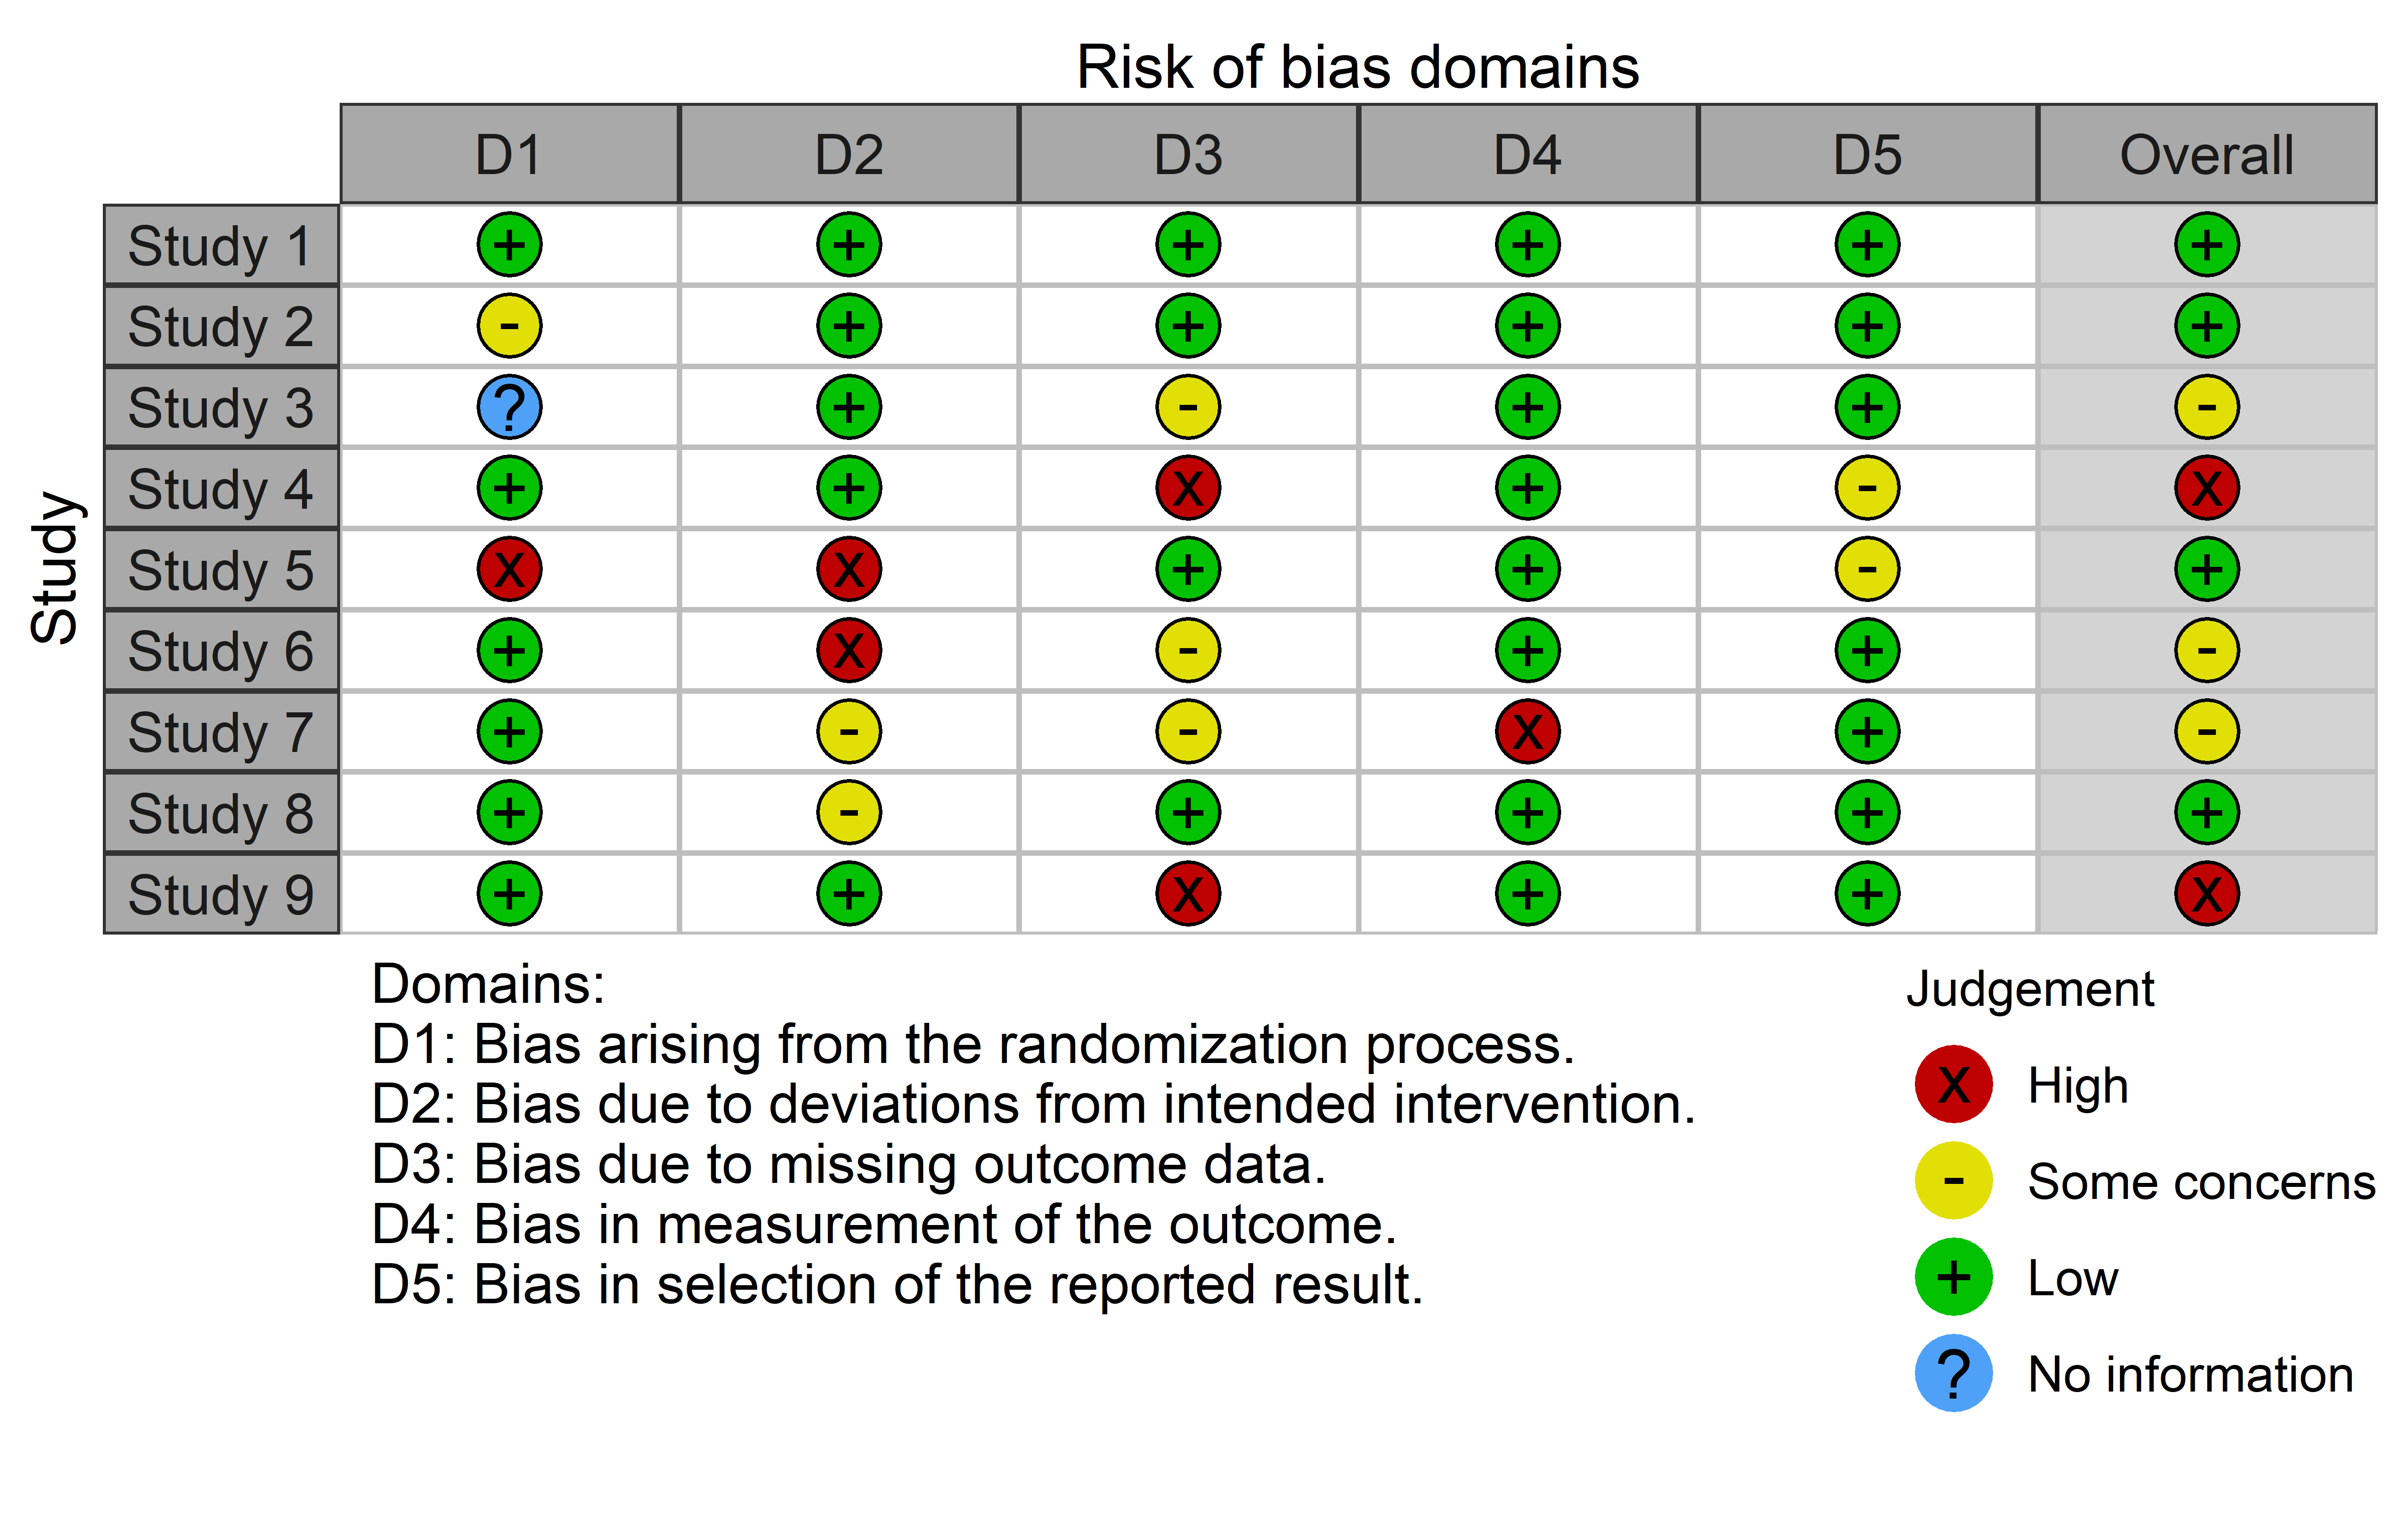
\includegraphics[width=1\linewidth]{figures/sys-rev-tools/example-rob-traffic-light-plot} \caption{Example risk of bias traffic light plot created using `robvis`}\label{fig:trafficplot}
\end{figure}

Similary, using the same data set, the summary barplot shown in Figure \ref{fig:summaryplot} is created using:

\begin{Shaded}
\begin{Highlighting}[]
\KeywordTok{rob_summary}\NormalTok{(}\DataTypeTok{data =}\NormalTok{ data_rob2,}
            \DataTypeTok{tool =} \StringTok{"ROB2"}\NormalTok{, }
            \DataTypeTok{overall =} \OtherTok{TRUE}\NormalTok{)}
\end{Highlighting}
\end{Shaded}

\begin{figure}
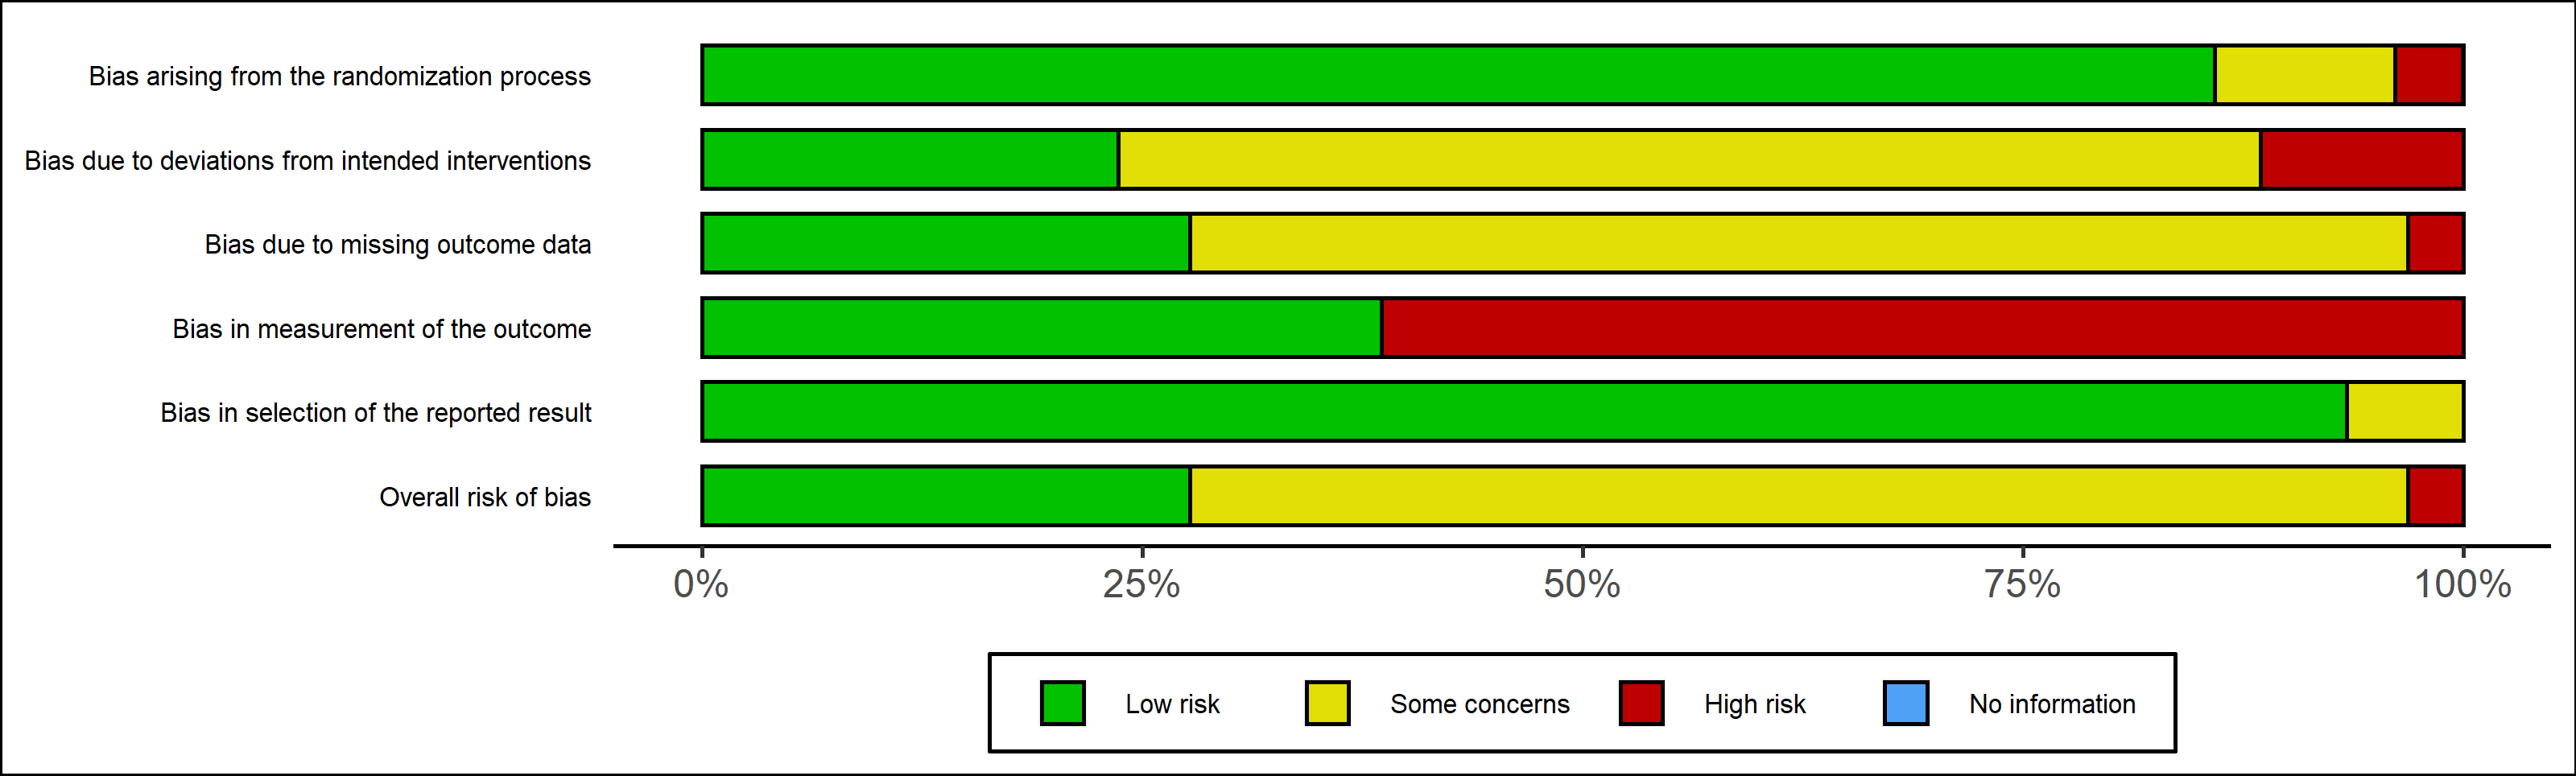
\includegraphics[width=1\linewidth]{figures/sys-rev-tools/example-rob-summary-barplot} \caption{Example risk of bias summary plot created using `robvis` and the example ROB2 dataset}\label{fig:summaryplot}
\end{figure}

A list of arguments available to the two functions in robvis are shown in Table \ref{tab:robvisarguments}

\begingroup\fontsize{9}{11}\selectfont

\begin{longtable}[t]{lcc>{\raggedright\arraybackslash}p{5cm}}
\caption{\label{tab:robvisarguments}Description of the arguments available in the two main `robvis` functions. ‘X’ indicates that the option is available for the respective function.}\\
\toprule
Argument & rob\_traffic\_light() & rob\_summary() & Description\\
\midrule
\endfirsthead
\caption[]{\label{tab:robvisarguments}Description of the arguments available in the two main `robvis` functions. ‘X’ indicates that the option is available for the respective function. \textit{(continued)}}\\
\toprule
Argument & rob\_traffic\_light() & rob\_summary() & Description\\
\midrule
\endhead

\endfoot
\bottomrule
\endlastfoot
\cellcolor{gray!6}{data} & \cellcolor{gray!6}{X} & \cellcolor{gray!6}{X} & \cellcolor{gray!6}{Defines the dataframe containing the summary (domain) level risk-of-bias assessments. See the text and Table 1 for the format expected by `robvis`}\\
tool & X & X & Defines the risk of bias assessment tool used. The RoB2 (`tool="ROB2"`), ROBINS-I (`tool="ROBINS-I"`), and QUADAS-2 (`tool="QUADAS-2"`) assessments tools are currently supported. Other tools can be visualised using the generic template (`tool = "Generic"`)\\
\cellcolor{gray!6}{colour} & \cellcolor{gray!6}{X} & \cellcolor{gray!6}{X} & \cellcolor{gray!6}{Defines the colour scheme for the plot. The default is `colour = "cochrane"` which uses the "Cochrane" (red, yellow, green) colours, while a preset option for a colour-blind friendly palette is also available (`colour = "colourblind"`). Alternatively, users can specify their own colour scheme e.g. `colour = c("\#f442c8", "\#bef441", "\#000000")`}\\
overall &  & X & Defines whether to include an additional bar showing the distibution of overall risk of bias judgements in the summary barplot figure. Default is `overall = FALSE`.\\
\cellcolor{gray!6}{weighted} & \cellcolor{gray!6}{} & \cellcolor{gray!6}{X} & \cellcolor{gray!6}{Defines whether weights should be used to produce the summary barplot figure. Default is `weighted = TRUE`, in line with current Cochrane Collaboration guidance.}\\
\addlinespace
psize & X &  & Defines the size of the points in the traffic light plot. Default is `psize = 20`.\\*
\end{longtable}
\endgroup{}

\hypertarget{reception-and-future-plans-1}{%
\subsection{Reception and Future Plans}\label{reception-and-future-plans-1}}

As of December 2020, \texttt{robvis} has been downloaded more than 8800 times. It has been well recieved but the systematic review community, and has been cited frequently in the published literature. A paper describing the tool was published in a special issue of Research Synthesis Methods focusing on data visualisation methods. A chapter on the tool has been incorporated in to the ``Doing Meta-Analysis in R'' online textbook.\textsuperscript{\protect\hyperlink{ref-mathias_harrer_2019_2551803}{65}}

While \texttt{robvis} is a stable package, a range of additional functionality could be added. At present, the number of tools with a specific template included in \texttt{robvis} is limited - adding additional templates is a priority. For example, a template for ROBIS, a tool for assessing risk of bias in systematic reviews, is in developement.\textsuperscript{\protect\hyperlink{ref-whiting2016robis}{66}} Additionally, the tool does not yet allow for the production of paired forest plots, where the risk-of-bias judgement is presented alongside each specific result included in the meta-analysis.\textsuperscript{\protect\hyperlink{ref-cochranechpt7}{48}} This was initially considered to be beyond the scope of the tool, as it involves the visualization of something other than risk-of-bias assessments. However, following user-driven demand, this functionality is in development and will be available in the near future. Finally, we would like to add similar functionality to that provided by the \texttt{metafor::reporter()} function, which generates a brief paragraph of text describing the results of a meta-analysis. The future \texttt{robvis::reporter()} function would provide a boilerplate description of the assessment tool used and the key domains at risk of bias.


%%%%% REFERENCES

% JEM: Quote for the top of references (just like a chapter quote if you're using them).  Comment to skip.
% \begin{savequote}[8cm]
% The first kind of intellectual and artistic personality belongs to the hedgehogs, the second to the foxes \dots
%   \qauthor{--- Sir Isaiah Berlin \cite{berlin_hedgehog_2013}}
% \end{savequote}

\setlength{\baselineskip}{0pt} % JEM: Single-space References

{\renewcommand*\MakeUppercase[1]{#1}%
\printbibliography[heading=bibintoc,title={\bibtitle}]}

\end{document}
